\documentclass[a4paper,12pt]{book}
\usepackage[utf8]{inputenc}
\usepackage[T1]{fontenc}
\usepackage[spanish,  es-tabla]{babel} % If you write in French
% \usepackage[english]{babel} % If you write in French
\usepackage{a4wide}
\usepackage{graphicx}
\usepackage{amsthm}
\usepackage{amssymb,amsmath,bbm}
\usepackage{array}
\usepackage{bm}
\usepackage{multirow}
\usepackage[footnote]{acronym}
\usepackage{subcaption}
%\usepackage{subfig}
\usepackage{tikz}
\usetikzlibrary{shapes,arrows}
\usepackage{multicol}
\usepackage{cancel}
\usepackage{pgfplots}
\usepackage{bigints}
\pgfplotsset{compat=newest}
\pgfplotsset{plot coordinates/math parser=false}
\newlength\figureheight
\newlength\figurewidth
\pgfkeys{/pgf/number format/.cd, set decimal separator={,\!}, 1000 sep={\,},}
\usepackage[export]{adjustbox}
\usepackage{ifthen}
\usepackage{ifpdf}
\ifpdf
\usepackage[pdftex]{hyperref}
\else
\usepackage{hyperref}
\fi
\usepackage{color}
\hypersetup{
colorlinks=true,
linkcolor=black,
citecolor=black,
urlcolor=black}
%\usepackage[table,xcdraw]{xcolor}
\renewcommand{\baselinestretch}{1.05}

% Extra packages added to this template by Enrique Flores 19/09/2022
%\usepackage[spanish, es-tabla]{babel}
%\usepackage[spanish, es-tabla]
\newcommand{\EFM}[1]{{\color{blue}{#1}}}
\newcommand{\LS}[1]{{\color{purple}{#1}}}
\newcommand{\TS}[1]{{\color{olive}{#1}}}
\usepackage{color, colortbl}
\usepackage{tikz}
\usepackage{soul}
\usepackage{marginnote}
\usepackage{amsmath}
\usepackage{cancel}


\usepackage{fancyhdr}
\pagestyle{fancy}
\fancyfoot{}
\fancyhead[LE,RO]{\bfseries\thepage}
\fancyhead[RE]{\bfseries\nouppercase{\leftmark}}
\fancyhead[LO]{\bfseries\nouppercase{\rightmark}}
\setlength{\headheight}{15pt}
\let\headruleORIG\headrule
\renewcommand{\headrule}{\color{black} \headruleORIG}
\renewcommand{\headrulewidth}{1.0pt}
\usepackage{colortbl}
\arrayrulecolor{black}
\fancypagestyle{plain}{
  \fancyhead{}
  \fancyfoot[C]{\thepage}
  \renewcommand{\headrulewidth}{0pt}
}
\makeatletter
\def\@textbottom{\vskip \z@ \@plus 1pt}
\let\@texttop\relax
\makeatother
\makeatletter
\def\cleardoublepage{\clearpage\if@twoside \ifodd\c@page\else%
  \hbox{}%
  \thispagestyle{empty}%
  \newpage%
  \if@twocolumn\hbox{}\newpage\fi\fi\fi}
\makeatother
\parskip=5pt

%Todas las imagenes del documento deben estar en esta carpeta

\graphicspath{{Figures/}}
\usepackage[capposition=bottom]{floatrow}
%backend=biber
%Bibliography setup
\usepackage[sorting=none]{biblatex}
\addbibresource{references.bib}
% \usepackage{natbib}
%\usepackage{bibtex}
%\usepackage{biblatex}

%\bibliography{references}
%\bibliographystyle{unsrt}

%\let\chaptername\relax

\begin{document}
\begin{titlepage}
\begin{figure}
    \centering
    \begin{subfigure}[h]{0.3\textwidth}
        
\includegraphics[width=1\textwidth, left]{logoUNED.png}
    \end{subfigure}
    \qquad\qquad\qquad\qquad
    \begin{subfigure}[h]{0.3\textwidth}
        
\includegraphics[width=1\textwidth, right]{escudoUNED.jpeg}
    \end{subfigure}

\end{figure}


\begin{center}
{\large Universidad Nacional de Educación a Distancia}\\[0.5cm]
{\large Escuela Técnica Superior de Ingeniería Informática}\\[0.5cm]
{\large Máster Universitario en Ingeniería de Sistemas y de Control}\\[0.5cm]
{\large Trabajo de Fin de Master}\\[0.5cm]

% Title
\rule{\linewidth}{0.5mm} \\[0.4cm]
{ \huge \bfseries \textsc{Implementación de filtros de Kalman para control de actitud en microcontrolador Raspberry Pi Pico} \\[0.4cm] }
\rule{\linewidth}{0.5mm} \\[1.5cm]

% Author and supervisor
\noindent
\begin{minipage}{0.4\textwidth}
  \begin{flushleft} \large
    \emph{Autor:}\\
Enrique \textsc{flores montoya}\\
  \end{flushleft}
\end{minipage}%
\begin{minipage}{0.4\textwidth}
  \begin{flushright} \large
    \emph{Directoras:} \\
    Raquel \textsc{Dormido}\\
    Natividad \textsc{Duró}
  \end{flushright}
\end{minipage}

\vfill

% Bottom of the page
{\today}

\end{center}
\end{titlepage}
\frontmatter

\chapter*{Abstract}

\noindent\rule[2pt]{\textwidth}{0.5pt}\\



\noindent\rule[2pt]{\textwidth}{0.5pt}\\
\clearpage
\chapter*{Agradecimientos}





\clearpage
\tableofcontents
\clearpage
%\listoffigures
\chapter*{Nomenclatura}

\begin{multicols}{2}

\begin{tabbing}
 XXX \= \kill% this line sets tab stop
 $\rho$ \> density \\
 $u$ \> streamwise velocity\\
 $v$ \> transverse velocity\\
 $p$ \> pressure \\
 $T$ \> temperature \\
 $e$ \> internal energy\\
 $h$ \> enthalpy\\
 $H$ \> total enthalpy\\
 $\mu$ \> viscous coefficient \\
 $\nu$ \> kinematic viscous coefficient \\
 $k$ \> thermal conductivity \\
 $c_p$ \> specific heat capacity \\
 $\gamma$ \> adiabatic index\\
 $a$ \> sound speed\\
 $r$ \> recovery factor\\
 $\mathcal{R}_g$ \> ideal gas constant \\
 $T_S$ \> Sutherland's constant \\
 $C$ \> (defined in equation \eqref{eq:constant_C}) \\
 $ $ \>     \\

 $\tau$ \>  shear stress\\
 $q$ \> heat transfer rate\\
 $u_\tau$ \> friction velocity\\
 $T_\tau$ \> friction temperature\\
 $ $ \>     \\

 $M$ \> Mach number \\
 $Pr$ \> Prandtl number \\
 $Pr_t$ \> turbulent Prandtl number \\
 $Re_L$ \> $L$-based Reynolds number \\
 $Re_\delta$ \> $\delta$-based Reynolds number \\
 $Re_\theta$ \> $\theta$-based Reynolds number \\
 $Re_x$ \> $x$-based Reynolds number \\
 $ $ \>     \\

 $\delta$ \> boundary layer thickness   \\
 $\delta_t$ \> thermal boundary layer thickness   \\
 $\delta^*$ \> displacement thickness   \\
 $\theta$ \> momentum thickness   \\
 $\theta_H$ \> total enthalpy thickness   \\
 $\mathcal{H}$ \> shape factor\\
 $ $ \>     \\

 $\nu_T$ \> eddy viscosity\\
 $\alpha_T$ \> turbulent thermal diffusivity\\
 $\kappa$ \> Von Karman constant\\
 $\kappa_h$ \> thermal Von Karman constant\\
 $c$ \> logarithmic profile constant    \\
 $c_h$ \> thermal logarithmic profile constant    \\
 $\Pi$ \> wake constant\\
 $\Pi_h$ \> thermal wake constant\\
 $ $ \>  \\

 $C_f$ \> skin-friction coefficient\\
 $St$ \> Stanton number\\
 $\hat{q}$ \> dimensionless heat flux\\
 $ $ \>     \\

 $x,y $\>  spatial coordinates  \\
 $X,Y $\>  Stewartson's transformation coordinates  \\
 $U,V $\>  transformed velocity components  \\
 $\eta$\> self-similar coordinate\\
 $\Psi$ \> stream function \\
 $f$ \> similarity function \\
 $\Theta$ \> dimensionless temperature \\
 $S$ \> enthalpy function \\
 $L$ \> plate length\\
 $ $ \>  \\

\textit{Subscript}\\
% $F$ \> Frozen flow \\
 $e$ \> external flow properties \\
 $i$ \> incompressible flow properties \\
 $w$ \> wall-evaluated conditions  \\
 $\text{eq}$ \> equilibrium properties \\
 $\infty$ \>freestream properties \\
 $t$ \>freestream stagnation properties \\
 $x,y$ \> spatial derivation in the physical \\
  \>  plane \\
 $X,Y$ \> spatial derivation in the transformed\\
  \>  plane \\
 $ $ \>  \\

\textit{Superscript}\\
 $+$ \> boundary-layer scaled properties \\
 $*$ \> non-dimensionalized quantities \\
 $\prime$ \> fluctuating flow properties \\
\end{tabbing}

\end{multicols}

\mainmatter
\pagestyle{fancy}
\clearpage

\chapter{Introducción}\label{chapter:Introduccion}

Los vehículos autónomos tales como los cuadricópteros han experimentado un intenso desarrollo en las últimas décadas. Su avance se ha visto impulsado por las mejoras en las baterías, los motores sin escobillas así como en el abaratamiento y la miniaturización de la electrónica. A día de hoy, existen un gran número de herramientas de propotipado accesibles al gran público tales como Arduino o Raspberry pi. Estos dispositivos se caracterizan por su flexibilidad, bajo coste y accesibilidad. Además, existen otros muchos microcontroladores disponibles en el mercado que se utilizan en aplicaciones de robótica tales como el ESP8266, el ATMEGA328 y el STM32.

La Raspberry pi Pico es un microcontrolador recientemente desarrollado y comercializado por Raspberry. Su uso está menos extendido que el de Arduino pero su potencia y capacidad de procesado son mucho mayores. Esto lo convierte en un microcontrolador más adecuado para aplicaciones de mayor nivel donde se requieren mayores frecuencias de reloj y un procesado de datos más complejo.

El control de los vehículos autónomos requiere estimar su posición y su actitud para poder enviar las señales de control a los actuadores. Para ello, estos sistemas integran diferentes sensores tales como medidores de altitud barométricos, IMUs (Inertial Measurement Unit), GPSs y cámaras de baja resolución. No obstante, en general, se necesita procesar los datos de los sensores para  estimar el estado del sistema. La mayoría de los vehículos utilizan filtros de Kalman para la estimación de la actitud \cite{zhang2005navigation, pettersson2015extended, trawny2005indirect}.


El filtro de Kalman fue desarrollado por Rudolf E. Kalman en 1960. En \cite{kalman1960new}, Kalman describe una solución recursiva para el problema del filtrado lineal de datos discretos. El filtro es un procedimiento matemático que opera por medio de un mecanismo de predicción y corrección (\url{https://www.kalmanfilter.net/default.aspx}). En esencia este algoritmo pronostica el nuevo estado a partir de su estimación previa
añadiendo un término de corrección proporcional al error de predicción, de tal forma que este último es minimizado estadísticamente.


Los filtros de Kalman tienen numerosas aplicaciones tecnológicas. Uno de los primeros usos del filtro de Kalman fue el procesado de los datos para  el guiado y el control de trayectoria de las naves en el programa Apollo. Desde ese momento, debido en gran parte al avance en el cálculo digital, el filtro de Kalman ha sido objeto de una extensiva investigación y aplicación, particularmente en el área de la navegación autónoma y asistida, en rastreo de misiles y en economía. El filtro se caracteriza por su bajo coste computacional y sus buenas propiedades recursivas. Es uno de los algoritmos de fusion de datos y sensores más comunes y más utilizados. 


El objetivo del presente trabajo es implementar un filtro de Kalman para la estimación de la actitud de un vehículo autónomo.


\chapter{Fundamentos Teóricos}\label{chapter:fundamentos}


\section{Sistemas de referencia}

\begin{figure}[h]
\centering
% \begin{tikzpicture}[scale=2]
% % Inertial frame
% % \draw[thick,->] (0,0) -- (1.5,0) node[anchor=north west]{$x$};
% % \draw[thick,->] (0,0) -- (0,1.5) node[anchor=south east]{$y$};
% % \draw[thick,->] (0,0) -- (-0.8,-0.8) node[anchor=north east]{$z$};
% % Body frame with rotation and offset
% \begin{scope}[rotate=30, xshift=1cm, yshift=1cm]
%     \draw[thick,->,blue] (0,0) -- (1,0) node[anchor=north]{$x_b$};
%     \draw[thick,->,blue] (0,0) -- (0,1) node[anchor=west]{$y_b$};
%     \draw[thick,->,blue] (0,0) -- (-0.5,-0.5) node[anchor=north east]{$z_b$};
% \end{scope}
% % Yaw angle
% \draw[dashed] (0,0) -- (1,0);
% \draw[thick,->,red] (0.5,0) arc (0:45:0.5) node[anchor=west]{$\psi$};
% % Pitch angle
% \draw[dashed] (0,0) -- (-0.5,-0.5);
% \draw[thick,->,red] (-0.3,-0.3) arc (-45:-90:0.5) node[anchor=east]{$\theta$};
% % Roll angle
% \draw[dashed] (0,0) -- (0,1);
% \draw[thick,->,red] (0,0.5) arc (90:45:0.5) node[anchor=south]{$\phi$};
% \end{tikzpicture}
\caption{Inertial and body frames with rotation and offset}
\end{figure}

En esta sección se presentan los sistemas de referencia empleados para definir la actitud de un vehículo aéreo. Los sistemas de referencia se denotan, de forma genérica por, $F(O,x,y,z)$ donde $(O)$ indica el origen y $(x,y,z)$ son los ejes del sistema de referencia. En la definición de la actitud de un vehículo es necesario considerar dos sistemas de referencia relevantes,

\subsection{Sistema de referencia inercial: $(O_I, x_I, y_I, z_I)$}

Es un sistema de referencia cartesiano inercial centrado en un punto arbitrario de la superficie terrestre, $O_I$. El eje $x_I$ apunta en la dirección del norte geodésico, el eje $y_I$ apunta en la dirección del este geodésico y el eje $z_I$ apunta en la dirección del centro de la tierra. Este sistema de referencia, en ocasiones denotado por NED (North-East-Down) se utiliza a menudo en para la navegación en aeronaves de pequeño tamaño. Generalmente, se toma el punto de despegue del vehículo como origen del sistema de coordenadas y se utiliza este sistema de referencia para describir la posición, la velocidad y la aceleración del vehículo con respecto a este punto.

\subsection{Sistema de referencia ejes cuerpo: $(O_b, x_b, y_b, z_b)$ }

El sistema de referencia ejes cuerpo $(O_b, x_b, y_b, z_b)$ esta centrado en el centro de gravedad del vehículo. El eje $x_b$ apunta hacia adelante y está contenido en el plano de simetría del vehículo, el eje $y_b$ apunta a estribor (hacia la derecha desde el punto de vista de un observador que mira en la dirección del eje $x_b$) y el eje $z_b$ apunta hacia abajo, en dirección al suelo, y esta también contenido en el plano de simetría del vehículo.

En los vehículos aéreos, las rotaciones alrededor de los ejes cuerpo se conocen respectivamente como balance, cabeceo y guiñada o \emph{roll, pitch} y \emph{yaw} por sus nombres en inglés. Estos ángulos describen la orientación del vehículo con respecto a los ejes inerciales $(O_I, x_I, y_I, z_I)$, lo que se conoce comúnmente como actitud del vehículo.


\section{Formalismos para describir la actitud}



Las rotaciones permiten pasar de unos sistemas de referencia a otros. Existen diferentes formalismos que se emplean para representar las transformaciones entre sistemas de referencia. El método más intuitivo para describir la orientación o actitud de un cuerpo en el espacio son los ángulos de Euler según la convención de Tait-Bryan. Sin embargo, los ángulos de Euler tienen ciertas limitaciones que hacen que los cuaternios sean el formalismo adoptado en los sistemas de estimación de la actitud. La descripción de la actitud mediante cuaternios puede traducirse a ángulos de Euler, lo que permite obtener un resultado más fácilmente interpretable.

\subsection{Ángulos de Euler}

\subsubsection{Fundamentos}

La forma más intuitiva de describir la actitud de un cuerpo en el espacio es mediante los ángulos de Euler. La orientación de un sistema de referencia con respecto a otro puede describirse mediante tres rotaciones sucesivas. Las rotaciones se representan mediante matrices ortonormales $3\times3$\footnote{Una matriz $M$ es ortogonal si y solo si $M^T=M^{-1}$ y además es ortonormal si cumple que su norma es la unidad, es decir, que el módulo de cada vector que la forma es la unidad.}. La composición de rotaciones se obtiene multiplicando matrices de rotación individuales y la transformación inversa viene dada por la matriz transpuesta de la matriz de rotación. El orden en el que se realizan las rotaciones alrededor de los diferentes ejes se denomina convención. Nótese que las rotaciones finitas no son conmutativas. Existen diferentes convenciones de ángulos de Euler. La convención utilizada para describir la orientación de aeronaves y vehículos espaciales es la convención de Tait-Bryan $zyx$. En otros campos científicos como la Física de Partículas o la Astronomía, son usuales convenciones distintas como la $zyz$ o la $zxz$. En aviónica, los ángulos de Euler se utilizan para describir la relación dentre los ejes inerciales $-I$ y los ejes cuerpo $-b$,\\

\begin{itemize}
    \item \textbf{Yaw} $\psi$: ángulo de rotación alrededor del eje $z_I$ del sistema de referencia inercial. El rumbo del vehículo viene dado por el ángulo formado entre la proyección el eje $x_b$ del vehículo sobre el plano formado por los ejes $x_I$ y $y_I$ y el eje $x_I$. La matriz de rotación asociada es,
    \begin{equation}
         C_\psi = \begin{bmatrix} \cos\psi & \sin\psi & 0 \\ -\sin\psi & \cos\psi & 0 \\ 0 & 0 & 1 \end{bmatrix}
    \end{equation}
    \item \textbf{Pitch} $\theta$: ángulo formado entre el plano $x_I-y_I$ y el eje $x_b$. La matriz de rotación correspondiente a este giro es,
    \begin{equation}
         C_\theta = \begin{bmatrix} \cos\theta & 0 & -\sin\theta \\ 0 & 1 & 0\\ \sin\psi & 0 & \cos\psi  \end{bmatrix}
    \end{equation}
    \item \textbf{Roll} $\phi$: ángulo de rotación alrededor del eje $x_b$. La matriz de rotación asociada a esta transformacióon viene dada por,
    \begin{equation}
         C_\phi= \begin{bmatrix} 1 & 0 & 0\\ 0 &\cos\psi & \sin\psi \\ 0 & -\sin\psi & \cos\psi  \end{bmatrix}
    \end{equation}
\end{itemize}

La matriz de rotación global se obtiene mediante la composición de las tres rotaciones \emph{yaw, pitch, roll} y viene dada por la multiplicación de las matrices $C_\psi$, $C_\theta$ y $C_\phi$. De esta manera, la matriz de rotación que permite transformar las componentes de un vector expresadas en ejes inerciales a ejes cuerpo viene dada por,
\begin{equation}
    C_I^b = C_\phi C_\theta C_\psi
\end{equation}
donde el orden de las rotaciones tiene lugar de derecha a izquierda. La expresión de la matriz de rotación resultante es,
\begin{equation}
         C_I^b= \begin{bmatrix}  \cos\theta\cos\psi & \cos\theta\sin\psi & -\sin\psi \\ \sin\phi\sin\theta\cos\psi - \cos\phi\sin\psi & \sin\psi\sin\theta\sin\psi + \cos\phi\cos\psi & \sin\phi\cos\theta \\ \cos\phi\sin\theta\cos\psi + \sin\phi\sin\psi & \cos\phi\sin\theta\sin\psi - \sin\phi\sin\psi & \cos\phi\cos\theta \end{bmatrix}
    \end{equation}
dado que la matriz $C_I^b$ es ortonormal, la transformación de un vector expresado en ejes cuerpo $(O_b,x_b,y_b,z_b)$ a ejes inerciales $(O_I,x_I,y_I,z_I)$ se realiza multiplicando por la matriz $C_b^I$, que satisface,
\begin{equation}
     C_b^I = (C_I^b)^{-1} = (C_I^b)^T
\end{equation}

\subsubsection{Propagación de ángulos de Euler}

El vector de velocidad angular del cuerpo con respecto al sistema de referencia inercial expresado en ejes cuerpo viene dado por,
\begin{equation}
    \mathbf{\omega} = \begin{bmatrix} \omega_x & \omega_y & \omega_z   \end{bmatrix} = \begin{bmatrix} p & q & r   \end{bmatrix}
\end{equation}
La relación entre la velocidad angular y la variación temporal de los ángulos de Euler viene dada por,
\begin{eqnarray}
    p & = &    \dot{\phi} - \dot{\psi}\sin\theta\\
    q & = & \dot{\theta}\cos\phi + \dot{\psi}\cos\theta\sin\phi\\
    r & = & -\dot{\theta}\sin\phi + \dot{\psi}\cos\theta\cos\phi
\end{eqnarray}

y la relación inversa se expresa como,
\begin{eqnarray}
    \dot{\phi} &=& p + (q\sin\phi + r\cos\phi)\tan\theta\\
    \dot{\theta} & =& q\cos\phi - r\sin\phi\\
    \label{eq:rolldot_pqr}\dot{\psi} & = & (q\sin\phi + r\cos\phi)\frac{1}{\cos\theta}
\end{eqnarray}

Nótese que la ecuación \eqref{eq:rolldot_pqr} es singular cuando el ángulo de asiento (pitch) es $\theta = \pm\pi/2$. Esto limita el uso de los ángulos de Euler para representar la actitud de un cuerpo haciendo que los cuaternios unitarios sean la alternativa escogida por la mayoría de sistemas de integración de la actitud.


\subsection{Cuaternios}
\subsubsection{Fundamentos}

Los cuaternios son un formalismo que permite describir la actitud de un cuerpo y las rotaciones entre diferentes sistemas de referencia. Un cuaternio esta formado por cuatro componentes,
\begin{equation}
    \mathbf{q} = \begin{bmatrix}
        q_1 & q_2 & q_3 &q_4
    \end{bmatrix}
\end{equation}
El cuaternio también puede expresarse como un número complejo con una componente real y cuatro componentes imaginarias,
\begin{equation}
    \mathbf{q} = q_0 + q_1\mathbf{i} + q_2\mathbf{j} + q_3\mathbf{k}
\end{equation}
El producto entre dos cuaternios $\mathbf{q_1} = \begin{bmatrix} q_0 & q_1 & q_2 &q_3\end{bmatrix}$ y $\mathbf{q_2} = \begin{bmatrix} a & b & c &d\end{bmatrix}$ puede expresarse como el producto de matrices,
\begin{equation}
    \mathbf{q_1}\cdot\mathbf{q_2} = \begin{bmatrix}q_0 & -q_1 & -q_2 & -q_3 \\ q_1 & q_0 & -q_3 & q_2 \\ q_2 & q_3 & q_0 & -q_1 \\ q_3 & -q_2 & q_1 & q_0  \end{bmatrix} \begin{bmatrix} a \\ b \\ c\\ d\end{bmatrix}
\end{equation}

Los cuaternios pueden usarse para describir las rotaciones entre sistemas de referencia. Un cuaternio de componentes $\begin{bmatrix} q_0 & q_1 & q_2 &q_3\end{bmatrix}$ representa un giro de un ángulo $\alpha$ alrededor de un eje $\mathbf{t} = \begin{bmatrix}t_x & t_y & t_z\end{bmatrix}$,
\begin{equation}
    \mathbf{q} = \left[\cos\frac{\alpha}{2},\>\mathbf{t}\sin\frac{\alpha}{2}\right]
\end{equation}
Sea $\mathbf{r_b}$ un vector cualquiera expresado en ejes cuerpo, este puede escribirse como un cuaternio cuya componente escalar es nula,
\begin{equation}
    \mathbf{r_b} = 0 + r_x\mathbf{i} + r_y\mathbf{j} + r_z\mathbf{k}
\end{equation}
Para expresar el vector $\mathbf{r_b}$ en ejes inerciales se aplica,
\begin{equation}
    \mathbf{r_I} = \mathbf{q\cdot r_b\cdot q^\star}
\end{equation}
donde $\mathbf{q^\star}$ denota el cuaternio conjugado de $\mathbf{q}$. Esta operación también puede expresarse de forma matricial como,
\begin{equation}
    \mathbf{r_I = \begin{bmatrix} 0 & 0 \\ 0 & C\end{bmatrix}r_b}
\end{equation}
donde $\mathbf{C}$ es la matriz de rotación entre el sistema de referencia ejes cuerpo y el sistema inercial $C_b^I$. La matriz $\mathbf{C}$ expresada en función de las componentes de $\mathbf{q}$ viene dada por,
\begin{equation}
    \mathbf{C} = \begin{bmatrix} (q_0^2 + q_1^2 - q_2^2 - q_3^2) & 2(q_1q_2 - q_0q_3) & 2(q_1q_3 + q_0q_2) \\ 2(q_1q_2 + q_0q_3) & (q_0^2 - q_1^2 + q_2^2 - q_3^2) & 2(q_2q_3 - q_0q_1) \\ 2(q_1q_3 - q_0q_2) & 2(q_2q_3 + q_0q_1) & (q_0^2 - q_1^2 - q_2^2 + q_3^2)     \end{bmatrix}
\end{equation}
de nuevo, la matriz $\mathbf{C}$ es ortonormal y su transpuesta puede utilizarse para rotar un vector expresado en el sistema de referencia inercial al sistema de referencia ejes cuerpo.

\subsubsection{Propagación de cuaternios}

Dado un sistema de ejes cuerpo $-b$ que rota con un vector velocidad angular $\mathbf{\omega} = \begin{bmatrix} p & q & r\end{bmatrix}$ con respecto al sistema de referencia inercial $-I$ y sea $\mathbf{q}$ el cuaternio que describe la orientación del sistema de referncia ejes cuerpo con respecto al sistema de referencia inercial, la variación temporal de $\mathbf{q}$ viene dada por,
\begin{equation}\label{eq:quaternion_prop}
    \dot{\mathbf{q}} = \frac{1}{2} \mathbf{q\cdot \Omega}
\end{equation}
donde $\mathbf{\Omega}$ se define como,
\begin{equation}
    \mathbf{\Omega} = \begin{bmatrix} 0 \\ p\\q\\r    \end{bmatrix}
\end{equation}
La ecuación \eqref{eq:quaternion_prop} puede expresarse en forma matricial como,
\begin{equation}
    \dot{\mathbf{q}} = \frac{1}{2}\begin{bmatrix}q_0 & -q_1 & -q_2 & -q_3 \\ q_1 & q_0 & -q_3 & q_2 \\ q_2 & q_3 & q_0 & -q_1 \\ q_3 & -q_2 & q_1 & q_0  \end{bmatrix}\begin{bmatrix} 0 \\ p\\q\\r    \end{bmatrix} = \frac{1}{2}\begin{bmatrix} -q_1 & -q_2 & -q_3 \\  q_0 & -q_3 & q_2 \\  q_3 & q_0 & -q_1 \\  -q_2 & q_1 & q_0  \end{bmatrix} \begin{bmatrix}  p\\q\\r    \end{bmatrix} = \frac{1}{2}\tilde{S}(\mathbf{q})\mathbf{\omega}
\end{equation}
Esta expresión puede reescribirse para expresarla como el producto entre una matriz $S(\mathbf{\omega})$ y el cuaternio $\mathbf{q}$,
\begin{equation}\label{eq:cuat_derv}
    \dot{\mathbf{q}} = \frac{1}{2}\begin{bmatrix}0 & -p & -q & -r \\ p & 0 & r & -q \\ q & -r & 0 & p \\ r & q & -p & 0  \end{bmatrix}\begin{bmatrix} q_0 \\ q_1\\q_2\\q_3    \end{bmatrix} = \frac{1}{2}S(\mathbf{\omega})\mathbf{q}
\end{equation}
La integración de la ecuación \eqref{eq:cuat_derv} en el tiempo proporciona la evolución de la orientación del cuerpo descrita por el cuaternio $\mathbf{q}$ en función de la velocidad angular del sistema $-b$ con respecto al sistema inercial $-I$, $\mathbf{\omega}$.

\subsubsection{Relación entre los cuaternios y los ángulos de Euler}
 
El cuaternio $\mathbf{q}$ que representa la orientación del sistema ejes cuerpo $-b$ con respecto al sistema inercial $-I$ puede expresarse en función de los ángulos de Euler $(\phi,\theta, \psi)$ como,
\begin{eqnarray}
    q_0 & = & \cos\frac{\phi}{2}\cos\frac{\theta}{2}\cos\frac{\psi}{2} + \sin\frac{\phi}{2}\sin\frac{\theta}{2}\sin\frac{\psi}{2}\\
    q_1 & = & \sin\frac{\phi}{2}\cos\frac{\theta}{2}\cos\frac{\psi}{2} - \cos\frac{\phi}{2}\sin\frac{\theta}{2}\sin\frac{\psi}{2}\\
    q_2 & = & \cos\frac{\phi}{2}\sin\frac{\theta}{2}\cos\frac{\psi}{2} + \sin\frac{\phi}{2}\cos\frac{\theta}{2}\sin\frac{\psi}{2}\\
    q_3 & = & \cos\frac{\phi}{2}\cos\frac{\theta}{2}\sin\frac{\psi}{2} - \sin\frac{\phi}{2}\sin\frac{\theta}{2}\cos\frac{\psi}{2}
\end{eqnarray}

Igualmente, a partir del cuaternio $\mathbf{q}$ que describe la orientación del sistema $-b$ podemos obtener los ángulos de Euler que definen la actitud del cuerpo,
\begin{eqnarray}
    \phi &=& \arctan\left[\frac{2(q_2q_3 + q_0q_1)}{1 - 2(q_1^2 + q_2^2)}\right]\\
    \theta &=& \arcsin\left[ 2(q_0q_2 - q_1q_3)\right]\\
    \psi &=& \arctan\left[\frac{2(q_1q_2 + q_0q_3)}{1 - 2(q_2^2 + q_3^2)}\right]
\end{eqnarray}
Las funciones arcotangente implementadas en los ordenadores solo producen resultados entre $\pm\pi/2$. Para poder generar todas las orientaciones es necesario sustituir la función \texttt{atan} por \texttt{atan2}, que tiene en cuenta el signo del numerador y del denominador. De nuevo, estas expresiones son singulares para $\theta\rightarrow \pm \pi/2$.



\chapter{Dispositivo experimental}\label{chapter:setup}

Para la determinación de la actitud del dispositivo se utilizará el sensor MPU 9250. Se trata de una IMU (Inertial Measurement Unit) que permite medir la aceleración, la velocidad angular y el campo magnético en las tres direcciones del espacio. A continuación se presentan los módulos de hardware utilizados así como la librería SDK para el control del hardware del microcontrolador Raspberry pi Pico.


\section{Sensor MPU 9250}
\begin{figure}[!h]
    \centering
	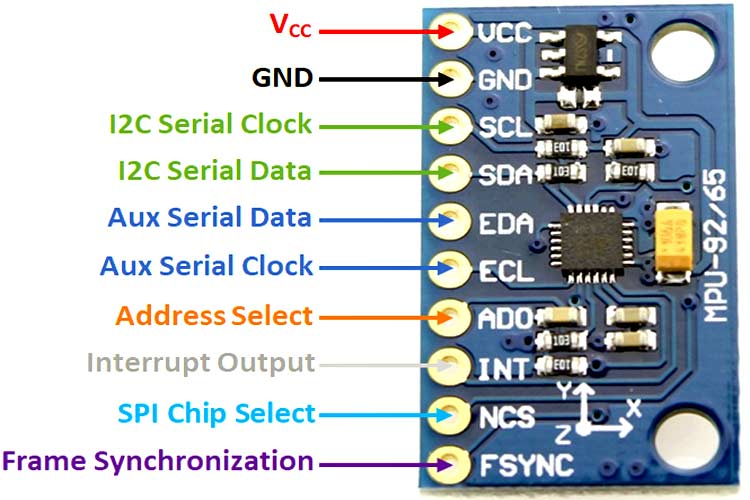
\includegraphics[width=0.3\linewidth]{MPU9250-Pin-Diagram.jpg}
 	\caption{Sensor MPU 9250}
 	\label{fig:mpu9250_pinout}
\end{figure}


El sensor MPU 9250 \cite{mpu9250datasheet} es un módulo multi-chip que consiste en en dos \emph{dies} integrados en un único paquete QFN. El primero de los \emph{dies} alberga un giróscopo y un acelerómetro de tres ejes. El segundo \emph{die} contiene el magnetómetro de tres ejes AK8963. Por tanto, el sensor MPU 9250 es un dispositivo de \emph{Motion Tracking} de 9 ejes que combina un giróscopo de 3 ejes, un acelerómetro de 3 ejes y un magnetómetro de 3 ejes así como un Procesador de Movimiento Digital (DMP).  

El MPU9250 puede conectarse a otros dispositivos mediante los buses de comunicación $\rm{I^2C}$ (frecuencia de acceso a registros de memoria de $400$~kz) y SPI (frecuencia de acceso a registros de memoria de $1$~MHz). El voltaje de operación del dispositivo es de $2.4$ -- $3.6$~V. El sensor cuenta con nueve conversores analógico-digitales de 16 bits para digitalizar las lecturas del giróscopo, el acelerómetro y el magnetómetro. Para la detección precisa de movimientos rápidos y lentos, los diferentes sensores cuentan con distintos rangos de medida programables: $\pm 250$, $\pm 500$, $\pm 1000$, $\pm 2000^\circ/\mathrm{sec}$ (dps) para el giróscopo, y  $\pm 2$~g, $\pm 4$~g, $\pm 8$~g, $\pm 16$~g para el acelerómetro. El magnetómetro tiene una rango de medida fijo de $\pm4800 \mu T$. El sensor cuenta con filtros digitales programables integrados, un reloj de precisión con una deriva del $1\%$ en el rango de temperatura $40^\circ$~C -- $85^\circ$~C, un sensor de temperatura e \emph{interrupts} programables. Se trata de un sensor de bajo coste (a partir de $1.59$ euros) lo que lo convierte en un buen candidato para la estimación de la actitud en vehículos autónomos y drones de pequeño tamaño y en aplicaciones académicas y de prototipado.


\section{Raspberry Pi Pico}

\begin{figure}[!h]
    \centering
	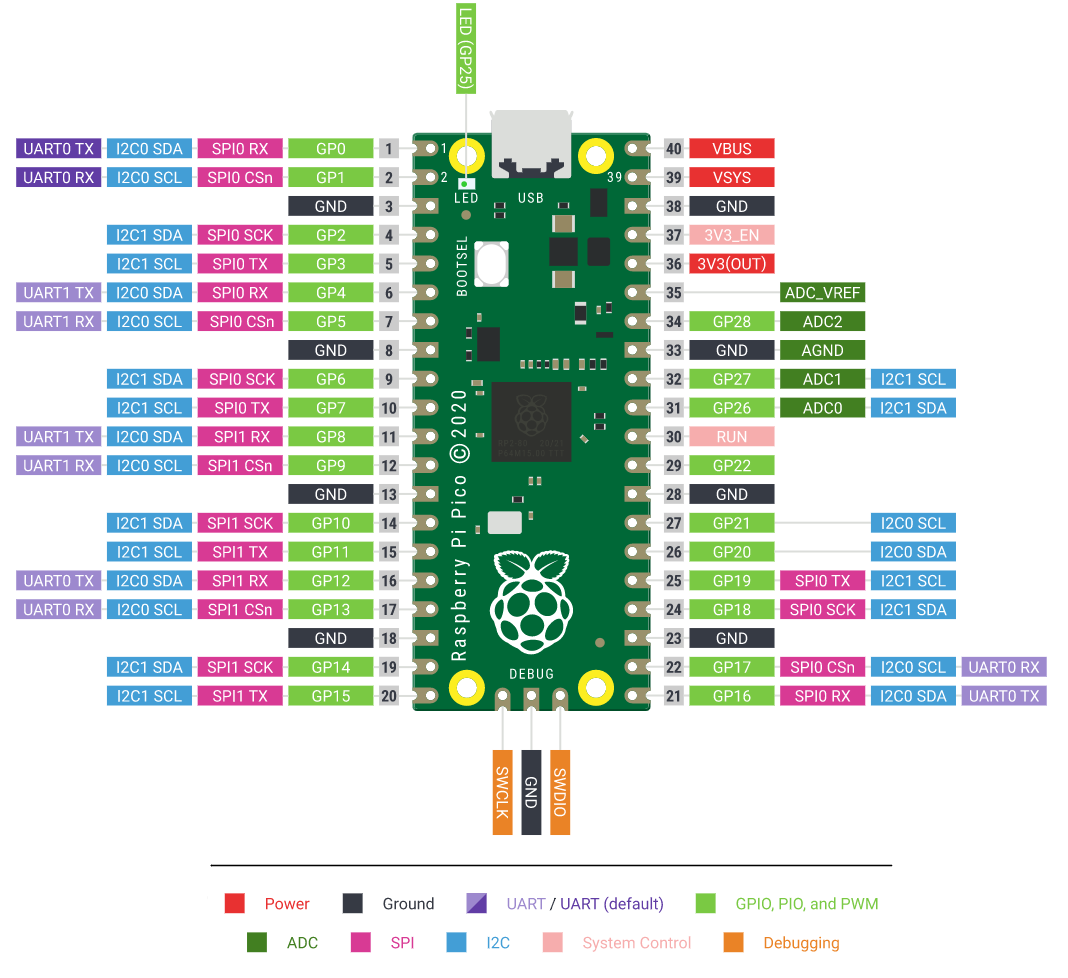
\includegraphics[width=0.8\linewidth]{raspberry_pi_Pico-R3-Pinout-narrow.png}
 	\caption{Raspberry pi Pico Pinout}
 	\label{fig:raspberry_pinout}
\end{figure}

La Raspberry pi Pico (\url{https://www.raspberrypi.com/products/raspberry-pi-pico/}) es un microcontrolador de alto rendimiento de tipo placa basado en el chip RP2040 diseñado por Raspberry Pi \cite{raspberrypiPico-datasheet}. El microcontrolador Raspberry pi Pico (RP$\pi$ Pico) embarca un procesador de doble núcleo dual-core ARM-CORTEX-M0+ (hasta 133 MHz) con una memoria SRAM interna de  264kB. La RP$\pi$ Pico cuenta con 2MB de memoria flash y un chip de \emph{power supply} que soporta voltajes de entrada de entre $1.8$ y $5.5$~V. El microcontrolador (ver figura \ref{fig:raspberry_pinout}) presenta 26 pines GPIO (General Purpose In-Out) incluyendo pines programables y soportando los protocolos de comunicación $\mathrm{I^2C}$ y SPI.

\subsection{Especificaciones (en inglés)}

\begin{itemize}
    \item 21 mm $\times$ 51 mm form factor
    \item RP2040 microcontroller chip designed by Raspberry Pi in the UK
    \item Dual-core ARM Cortex-M0+ processor, flexible clock running up to 133 MHz 264kB on-chip SRAM
    \item 2MB on-board QSPI flash
    \item 26 multifunction GPIO pins, including: 3 analogue inputs, 2 UART, 2 SPI controllers, 2 I2C controllers, 16 PWM channels, 1 USB 1.1 controller and PHY with host and device support, and 8 Programmable I/O (PIO) state machines for custom peripheral support
    \item Supported input power 1.8–5.5V DC
    \item Operating temperature -20°C to +85°C
    \item Drag-and-drop programming using mass storage over USB
    \item Low-power sleep and dormant modes
    \item Temperature sensor
    \item Accelerated integer and floating-point libraries on-chip
\end{itemize}




\section{Librerías}

La Rapsberry pi Pico puede programarse en MicroPython \cite{micropython-raspberrypiPico} o en C/C++ \cite{c/c++-raspberrypiPicot}. En el presente trabajo se ha optado por la programación en C/C++. Para empezar a programar la Raspberry pi Pico en C/C++ es necesario definir un \emph{environment} e instalar una serie de librerías tales como SDK, OpenOCD, GDB y picoprobe. El proceso de instalación y los pasos a seguir para configurar el \emph{environment} están descritos en \cite{c/c++-raspberrypiPicot}.


La librería más importante es la librería SDK del chip RP2040 (\url{https://raspberrypi.github.io/pico-sdk-doxygen/}) \cite{c/c++-raspberrypiPicot, sdk-raspberrypiPico}. La librería SDK (Software Development Kit) proporciona \emph{headers}, funciones y métodos para escribir programas en dispositivos basados en el chip RP2040 tales como la Raspberry pi Pico. Estos métodos permiten controlar distintos elementos del hardware de la Raspberry pi Pico tales como los buses I2C, SPI y los \emph{timers}.

Un único programa se ejecuta en el dispositivo cada vez bajo el método convencional \texttt{main()}. El sistema soporta las librerías estándar de C/C++ e incluye múltiples APIs (Application Programming Interface) para acceder al hardware del RP2040, inclutendo DMA, IRQs y una amplia variedad de pines programables y periféricos de función definida. Así mismo, la SDK provee librerías de alto nivel para manejar temporizadores, USB, sincronizaciones y programación multi-núcleo. La librería SDK utiliza CMake para compilar.



\chapter{Caracterización de los sensores}\label{chapter:calibration}

{\color{red}
\section{Generalidades}

\subsection{Random walk}

Los sensores están sometidos a diferentes fuentes de ruido que afectan a los resultados obtenidos a la hora de estimar las variables de estado del sistema. El error en los sensores es especialmente relevante cuando las mediciones de los sensores se integran en el tiempo. Cuando una señal con ruido se integra en el tiempo los errores se van acumulando dando lugar a una deriva \emph{drift} en la integral de la señal. 

\subsection{Dealineación interna de los sensores}

}

\section{Calibración del giróscopo.}


La calibración del giróscopo se ha realizado en este caso utilizando un tiempo de muestreo de $50$~ms y un rango de medida de $\pm1000\>\mathrm{^\circ/s}$. La calibración del giróscopo consiste principalmente en determinar los valores del bias. Para ello se miden los valores de la velocidad en los tres ejes con el sensor estático. El bias en cada dirección se determina calculando el valor medio de la señal. La figura \ref{fig:gyro_bias} representa los valores de la velocidad angular medidos durante un intervalo de tiempo de $30$~s con y sin bias.

\begin{figure}[!h]
    \centering
	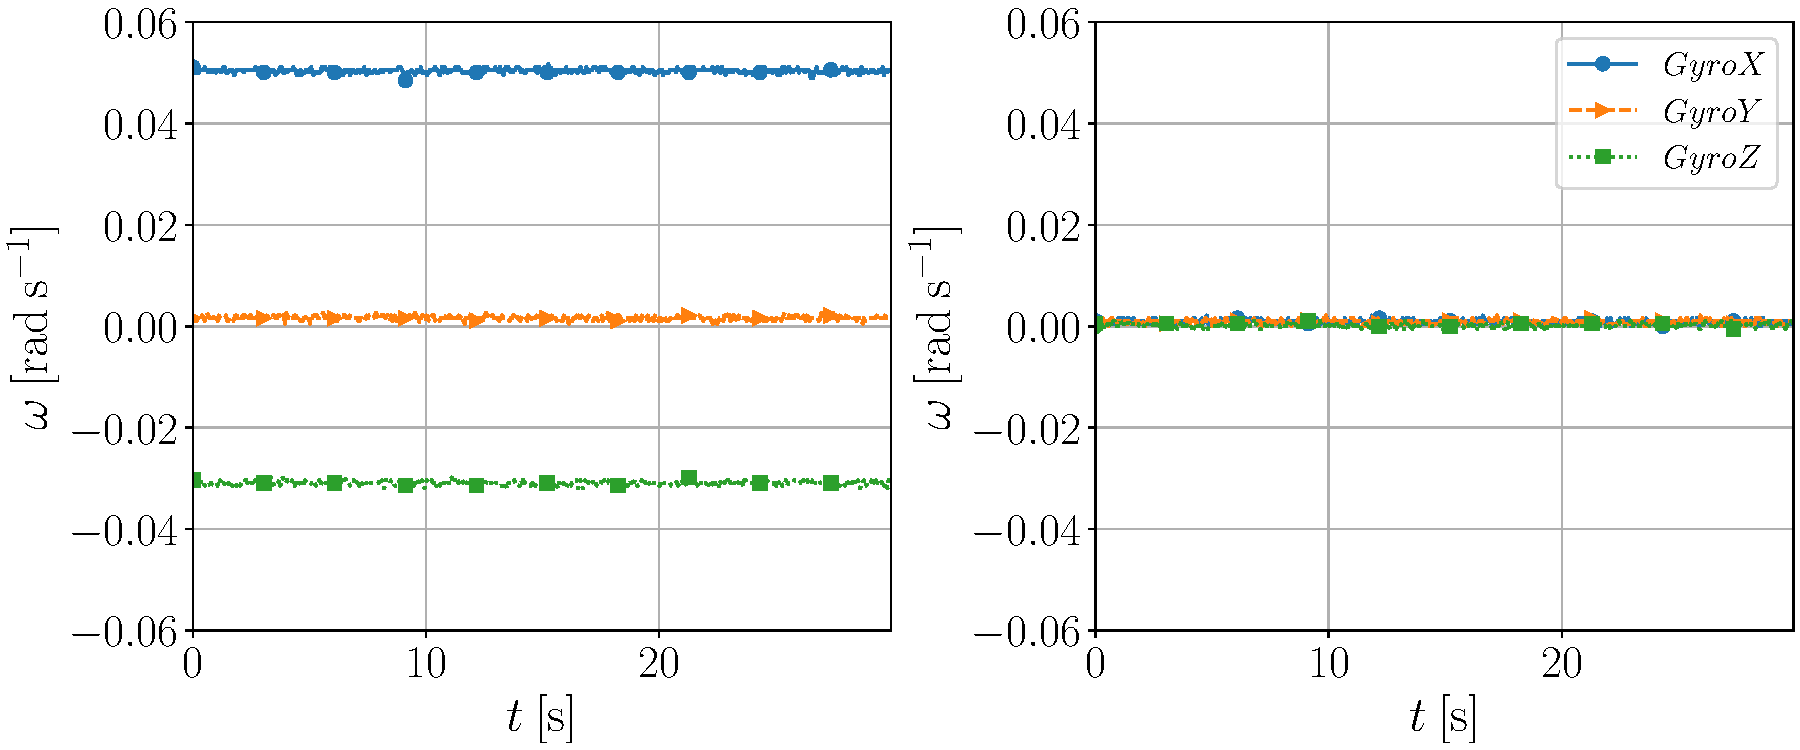
\includegraphics[width=0.9\linewidth]{gyro_bias.pdf}
 	\caption{Mediciones estáticas del giroscopipo: con bias (izquierda) y sin bias (derecha)}
 	\label{fig:gyro_bias}
\end{figure}

La tabla \ref{tab:gyro_bias} representa los valores del bias y de la desviación típica de las lecturas del giróscopo en cada eje.

\begin{table}[!h]
\centering
\begin{tabular}{c|c|c}
\textbf{Eje} &
  \textbf{\begin{tabular}[c]{@{}c@{}}Bias\\ {[}rad/s{]}\end{tabular}} &
  \textbf{\begin{tabular}[c]{@{}c@{}}STD \\ {[}rad/s{]}\end{tabular}} \\ \hline
$\omega_x$ & $0.0504$ & $4.199\times 10^{-4}$ \\
$\omega_y$ & $0.0017$ & $4.204\times 10^{-4}$ \\
\multicolumn{1}{l|}{$\omega_z$} &
  \multicolumn{1}{l|}{$-0.0309$} &
  \multicolumn{1}{l}{$4.391\times 10^{-4}$}
\end{tabular}
\vspace{1em}
\caption{Caracterización del giróscopo.}
\label{tab:gyro_bias}
\end{table}


\section{Calibración del acelerómetro}

\begin{figure}[!h]
    \centering
	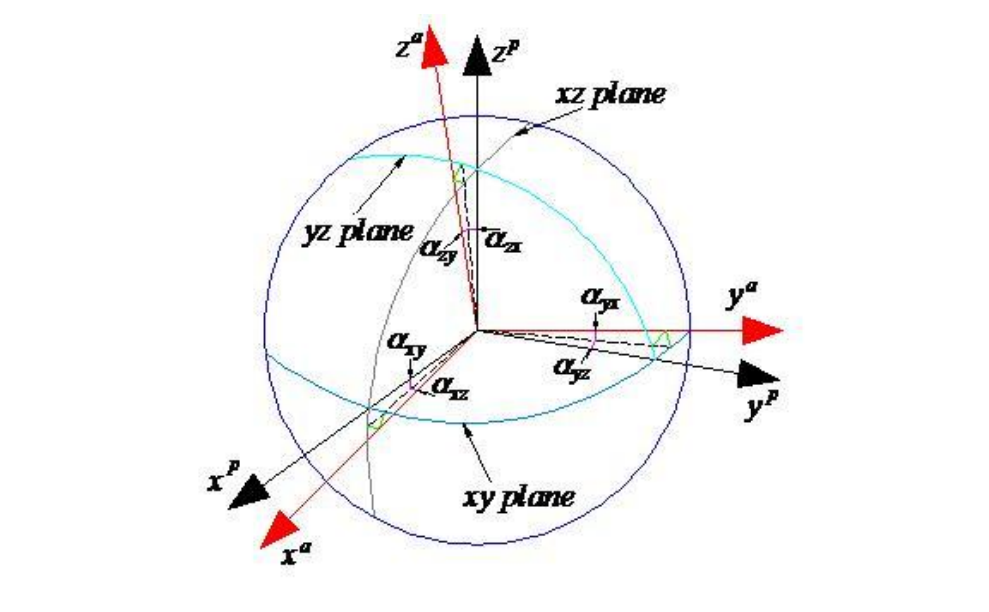
\includegraphics[width=0.6\linewidth]{axis_misalignment.png}
 	\caption{Errores de alineamiento entre los ejes del acelerómetro y el sistema de ejes cuerpo.}
 	\label{fig:axis_misalignment}
\end{figure}
\begin{table}[!h]
\centering
\begin{tabular}{lllllllll}
\multicolumn{1}{c}{$k_x$} &
  \multicolumn{1}{c}{$k_y$} &
  \multicolumn{1}{c}{$k_z$} &
  \multicolumn{1}{c}{\begin{tabular}[c]{@{}c@{}}$a_{yz}$\\ {[}rad{]}\end{tabular}} &
  \multicolumn{1}{c}{\begin{tabular}[c]{@{}c@{}}$a_{zy}$\\ {[}rad{]}\end{tabular}} &
  \multicolumn{1}{c}{\begin{tabular}[c]{@{}c@{}}$a_{zx}$\\ {[}rad{]}\end{tabular}} &
  \multicolumn{1}{c}{\begin{tabular}[c]{@{}c@{}}$b_{x}$\\ $\mathrm{[m\>s^{-2}]}$\end{tabular}} &
  \multicolumn{1}{c}{\begin{tabular}[c]{@{}c@{}}$b_{y}$\\ $\mathrm{[m\>s^{-2}]}$\end{tabular}} &
  \multicolumn{1}{c}{\begin{tabular}[c]{@{}c@{}}$b_{z}$\\ $\mathrm{[m\>s^{-2}]}$\end{tabular}} \\ \hline
0.9957 &
  0.9898 &
  0.9666 &
  0.01423 &
  0.05225 &
  0.00074 &
  -0.9497 &
  -1.5212 &
  -1.5564
\end{tabular}
\caption{Parámetros de calibración del acelerómetro}
\label{tab:acc_calibration}
\end{table}

\begin{figure}[!h]
    \centering
	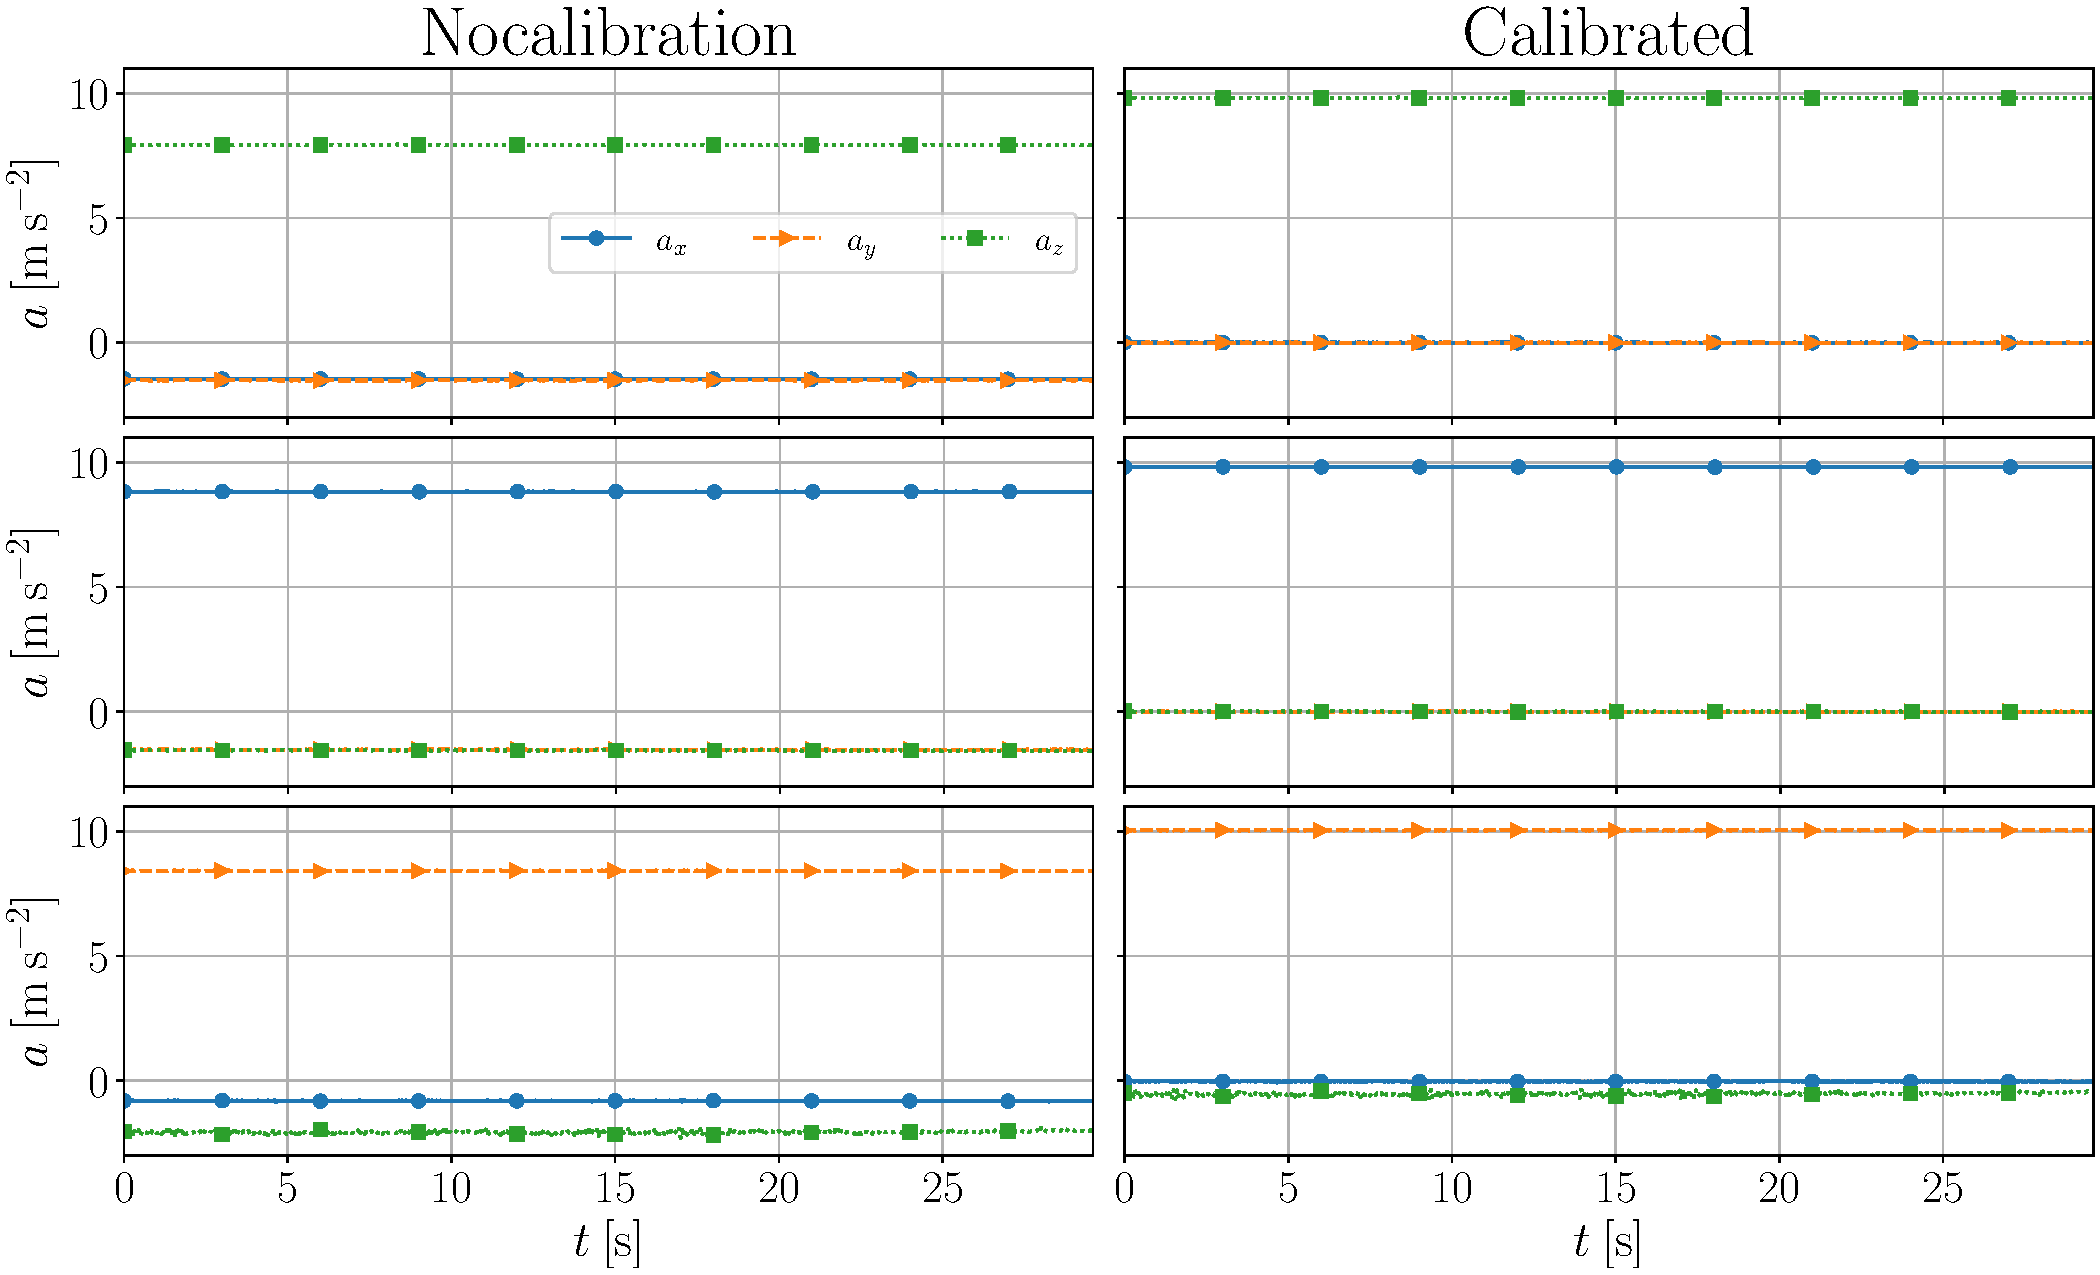
\includegraphics[width=0.9\linewidth]{accel_cal.pdf}
 	\caption{Lecturas estáticas del acelerómetro para tres orientaciones diferentes previas a la calibración (izquierda) y posteriores a la calibración (derecha).}
 	\label{fig:accel_cal}
\end{figure}
Idealmente, las direcciones en las que el sensor mide la aceleración deberían de ser ortogonales entre sí. Sin embargo, debido a las imprecisiones en la construcción de la IMU, a menudo existen desajustes en el alineamiento de los ejes. Esto se traduce en una falta de ortogonalidad entre los ejes del sensor que causa errores en las lecturas del acelerómetro. La figura \ref{fig:axis_misalignment} esquematiza los errores de desalineamineto entre los ejes del sensor y el sistema de ejes cuerpo $-b$. En esta sección se presenta un método para corregir los errores de alineamiento mediante de una calibración estática del acelerómetro. Los detalles del método pueden encontrarse en \cite{tee2011triaxial}. En principio, se requiere conocer un total de seis ángulos de desviación, $(a_{xy},  a_{xz}, a_{yx}, a_{yz}, a_{zx}, a_{zy})$, entre los ejes del sensor y los ejes cuerpo para corregir los errores de ortogonalidad. Sin embargo, \cite{skog2006calibration} mostraron que el modelo de error puede simplificarse si se asume que el eje $x_b$ coincide con el eje $x_a$. Las lecturas del sensor pueden modelarse de acuerdo al siguiente modelo de error,
\begin{equation}\label{eq:acc_calibration}
    v_i = ST^{-1}g_i + b + \epsilon
\end{equation}
donde $v_i$ es una lectura bruta, $i$, del acelerómetro, $S$ es una matriz diagonal que contiene los factores de escala, $T$ es la matriz de desalineación, $b$ es el bias constante de cada uno de los ejes del sensor y $\epsilon$ es el ruido. El vector $g_i$ es el vector de gravedad. La matriz $T$  permite transformar un vector expresado en ejes acelerómetro $-a$ a ejes cuerpo $-b$. Su expresión es,
\begin{equation}
    T = \begin{bmatrix} 1 & -a_{yz} & -a_{zy} \\ 0 & 1 & -a_{zx} \\ 0 &0&1   \end{bmatrix}
\end{equation}
A partir de la ecuación \eqref{eq:acc_calibration}, un total de nueve parámetros recogidos en \eqref{eq:acc_calib_params} deben ser determinados para corregir las lecturas del sensor.
\begin{equation}\label{eq:acc_calib_params}
    \begin{bmatrix} k_x & k_y & k_z &a_{yz} & a_{zy} & a_{zx} & b_x & b_y & b_z    \end{bmatrix}
\end{equation}
La ecuación \eqref{eq:acc_calibration} puede expandirse para obtener,
\begin{equation}\label{eq:acc_calibration_expanded}
    \begin{bmatrix} v_x \\ v_y \\ v_z    \end{bmatrix}_i = \begin{bmatrix} b_x + k_x g_{xi} + a_{yz}k_xg_{yi} - k_xg_{zi}(a_{zy} - a_{yz}a_{zx}) \\ b_y + k_y g_{yi} + a_{zx}k_y g_{zi} \\ b_z + k_zg_{zi}\end{bmatrix}_i
\end{equation}
El subíndice $-i$ denota la muestra $i$. Por tanto, utilizando un número $i$ de muestras correspondiente al número de incógnitas en cada eje, la ecuación \eqref{eq:acc_calibration_expanded} puede descomponerse en tres sistemas lineales de ecuaciones,
\begin{equation}
    \begin{bmatrix} v_{z1} \\ v_{z2}   \end{bmatrix} = \begin{bmatrix} 1& g_{z1} \\ 1& g_{z2}    \end{bmatrix} \begin{bmatrix} b_z \\ k_z    \end{bmatrix}
\end{equation}
\begin{equation}
    \begin{bmatrix} v_{y1}\\ v_{y2} \\ v_{y3}   \end{bmatrix} = \begin{bmatrix} 1& g_{y1} & g_{z1} \\ 1& g_{y2} & g_{z2} \\ 1 & g_{y3} & g_{z3}    \end{bmatrix} \begin{bmatrix} b_y \\ k_y \\ k_{yzx}   \end{bmatrix}
\end{equation}
\begin{equation}
    \begin{bmatrix} v_{x1}\\ v_{x2} \\ v_{x3} \\ v_{x4}   \end{bmatrix} = \begin{bmatrix} 1&  g_{x1} & g_{y1} & -g_{z1} \\ 1&g_{x2} &  g_{y2} & -g_{z2} \\ 1 &g_{x3} &  g_{y3} & -g_{z3}  \\ 1 &g_{x4} &  g_{y4} & -g_{z4}   \end{bmatrix} \begin{bmatrix} b_x \\ k_x \\ k_{xyz} \\ k_{xzy}   \end{bmatrix}
\end{equation}
donde
\begin{eqnarray}
    a_{zx} &=& \frac{k_{yzx}}{k_y}\\
    a_{yz} &=& \frac{k_{xyz}}{k_x}\\
    a_{zy} &=& \frac{k_{xzy}}{k_x} - a_{yz}a_{zx}
\end{eqnarray}
Para determinar los coeficientes de calibración del acelerómetro \eqref{eq:acc_calib_params} es necesario realizar $n$ mediciones del campo gravitatorio en $n$ orientaciones diferentes para las que se conozca el valor teórico de la dirección del vector de gravedad $\mathbf{g}$. Siendo $k$ el número de incógnitas por eje y $n$ el número de orientaciones evaluadas, existen un total de,
\begin{equation}
    \mathcal{C} = \frac{n!}{k!(n - k)!}
\end{equation}
combinaciones de medidas por cada eje para calcular los coeficientes de calibración. Aumentando el número de direcciones evaluadas $n$ es posible reducir el error en la estimación de \eqref{eq:acc_calib_params}. La tabla \ref{tab:acc_calibration} muestra los parámetros de calibración obtenidos tras haber evaluado cuatro orientaciones del sensor. Nótese que los valores de los factores de escala son adimensionales y pueden utilizarse para reescalar el módulo total del vector gravedad.

La figura \ref{fig:accel_cal} representa las lecturas del sensor en tres orientaciones distintas junto con 



\section{Calibración del magnetómetro.}

\begin{table}[!h]
\centering
\begin{tabular}{ccccccccc}
Localización &
  \begin{tabular}[c]{@{}c@{}}Latitud \\ {[}N{]}\end{tabular} &
  \begin{tabular}[c]{@{}c@{}}Longitud \\ {[}W{]}\end{tabular} &
  \begin{tabular}[c]{@{}c@{}}$h_x^I$\\ {[}nT{]}\end{tabular} &
  \begin{tabular}[c]{@{}c@{}}$h_y^I$\\ {[}nT{]}\end{tabular} &
  \begin{tabular}[c]{@{}c@{}}$h_z^I$\\ {[}nT{]}\end{tabular} &
  \begin{tabular}[c]{@{}c@{}}$\delta h_x^I$\\ {[}nT{]}\end{tabular} &
  \begin{tabular}[c]{@{}c@{}}$\delta h_y^I$\\ {[}nT{]}\end{tabular} &
  \begin{tabular}[c]{@{}c@{}}$\delta h_z^I$\\ {[}nT{]}\end{tabular} \\ \hline
Madrid &
  40° 25' 10" &
  3° 41' 31 &
  25749.4 &
  97.1 &
  36931.8 &
  131 &
  94 &
  157 \\
Toulouse &
  43° 36' 16" &
  1° 26' 39" &
  23869.8 &
  637.5 &
  39984.3 &
  131 &
  94 &
  157
\end{tabular}
\caption{Componentes del vector del campo magnético terrestre en ejes inerciales (NED) para dos localizaciones}
\label{tab:vector_magnetico}
\end{table}

El magnetómetro actúa como una brújula, proporcionando las tres componentes del vector del campo magnético terrestre medidas en ejes cuerpo $-b$.
\begin{equation}
    \mathbf{h}_b = \begin{bmatrix} h_x,\>h_y\>h_z    \end{bmatrix}_b
\end{equation}
El vector en ejes cuerpo debe ser transformado a ejes inerciales para poderlo comparar con la dirección del campo magnético terrestre en esa posición, que es un vector de referencia conocido. La dirección del vector del campo magnético terrestre varía a lo largo de la superficie terrestre pero puede considerarse constante para pequeños desplazamientos. A partir de las coordenadas de un punto de la superficie terrestre es posible obtener los valores de las componentes del vector del campo magnético utilizando herramientas tales como  \url{https://www.ngdc.noaa.gov/geomag/calculators/magcalc.shtml?#igrfwmm}. En la tabla \ref{tab:vector_magnetico} se recogen las componentes del campo magnético para dos localizaciones distintas junto con sus incertidumbres.

La comparación entre las lecturas del magnetómetro y el valor de referencia del campo magnético puede utilizarse para estimar la actitud del sistema de referencia ejes cuerpo $-b$. En contraste con el acelerómetro, el vector de referencia del campo magnético tiene componentes no nulas en el plano $x_Iy_I$ por lo que permite estimar el ángulo de guiñada $\psi$. Otra de las ventajas del magnetómetro es que sus medidas no se ven afectadas por las aceleraciones externas, que sí afectan a las lecturas del acelerómetro.

A día de hoy existen diferentes tipos de sensores del campo magnético basados en diferentes tecnologías. Por una parte podemos encontrar los sensores magnetorresistivos anisotrópicos (AMR por sus siglas en inglés). En este tipo de sensores existen elementos resistivos cuya resistencia efectiva cambia cuando son sometidos a un campo magnético. Su sensibilidad al campo magnético depende de la dirección del campo magnético incidente con respecto a la orientación del elemento magnetorresistivo, de ahí la denominación de anisotrópicos. Para la medición del campo magnético es necesario disponer cuatro elementos magnetorresistivos en configuración de puente de Wheatstone y medir el voltaje de salida. Es posible encontrar más detalles sobre esta tecnología en \cite{renaudin2010complete, freitas2007magnetoresistive}.

Por otra parte se encuentran lo sensores magnéticos de efecto Hall \cite{ramsden2011hall}. Los sensores magnéticos de efecto Hall son dispositivos electrónicos que detectan la presencia de un campo magnético utilizando el efecto Hall, descubierto por el físico estadounidense Edwin Hall en 1879. {\color{red}El efecto Hall se refiere al fenómeno de generar un potencial de voltaje en un conductor cuando se coloca en un campo magnético perpendicular y fluye una corriente a través de él.} Los sensores de efecto Hall consisten en una delgada tira de material semiconductor (como arseniuro de galio o silicio) a través de la cuál se hace pasar una corriente eléctrica. Al aproximar el sensor a un campo magnético perpendicular a la dirección de la corriente, se generará un voltaje proporcional al producto de la fuerza del campo magnético y la corriente. Conociendo el valor de la corriente, es posible calcular la fuerza del campo magnético. De entre las diferentes tecnologías de detección del campo magnético, los sensores de efectao Hall son los más extendidos. Una de las principales razones es que es posible producir sensores de gran calidad utilizando las técnicas convencionales de construcción de circuitos integrados. Esto permite integrar el sensor dentro de un chip de manera sencilla y barata. {\color{red}Los sensores de efecto Hall se utilizan ampliamente en una variedad de aplicaciones, incluyendo sistemas de control automotriz e industrial, robótica y electrónica de consumo. Son preferidos sobre otros tipos de sensores magnéticos en muchas aplicaciones porque son altamente sensibles, tienen un tiempo de respuesta rápido y no se ven afectados por factores ambientales como la temperatura, la humedad o la vibración.}

No obstante, el magnetómetro sufre de una serie de limitaciones que hacen que su calibración sea extremadamente importante para poderlo utilizar de forma efectiva en la estimación de la actitud del vehículo. Una descripción exhaustiva sobre las fuentes de error en los sensores de campo magnético magnetorresistivos puede encontrarse en \cite{renaudin2010complete}. De forma resumida, este tipo de sensores están sometidos a errores en los factores de escala asociados a la falta de proporcionalidad entre la salida del sensor y el campo magnético detectado, errores de offset debido a la presencia de campos parásitos, errores debido a la sensibilidad cruzada entre ejes o desalineamiento y, finalmente, a errores debido al ruido. De entre las fuentes de error que causan errores de offset y de desalineamiento podemos destacar los errores de hierro. Los errores de hierro están causados por las perturbaciones magnéticas originadas por la presencia de materiales ferromagnéticos y sistemas electromagnéticos en las proximidades del sensor. Estos errores están causados por los diferentes elementos de la planta donde se instala el sensor y dependen por tanto de su configuración. Esto hace que la calibración del sensor sea diferente en función de si este se instala en un placa de prototipado o en la planta final. Los errores de hierro se clasifican a su vez en errores de hierro duro y blando. Los errores de hierro duro están causados por fuentes de campo magnético cuyas componente del campo magnético son constantes en todas la direcciones. En otras palabras, son perturbaciones del campo magnético generadas por los diferentes subsistemas electrónicos presentes en las proximidades del sensor y que no dependen del campo magnético terrestre. Por otra parte, los errores de hierro blando surgen de la interacción entre el campo magnético terrestre y los elementos ferromagnéticos presentes en las proximidades del sensor. Estas perturbaciones tienen una naturaleza más compleja ya que dependen de la dirección del campo magnético terrestre incidente y, por tanto, de la orientación del sensor.


% \begin{itemize}
%     \item Error del Factor de Escala: Estos son errores que corresponden a fallas en la proporcionalidad de la salida de los sensores con respecto al campo magnético detectado.
%     \item Error de Offset: Estos son errores constantes que corresponden a la mala alineación de los puentes Wheatstone que componen el magnetómetro. 
%     \item Error de Sensibilidad: La sensibilidad de los elementos AMR varía con la amplitud del campo magnético medido. Esto resulta en un error en la escala de la salida de los sensores. Esto también puede compensarse con calibración y depende de la ubicación en lugar de la montura o el sensor real. Esto significa que la calibración para este tipo de errores debe realizarse en cada nueva ubicación. La calibración puede ser errónea si la magnitud del campo magnético está fuera del rango de calibración.
%     \item Sensibilidad Cruzada de Ejes: Con el tiempo, la exposición a un campo magnético hace que los elementos AMR se magneticen. Esta magnetización es desigual, lo que resulta en una mala alineación de los tres ejes del magnetómetro. Esto puede remediarse desmagnetizando los elementos AMR. Según \cite{renaudin2010complete}, esto se hace a menudo enrollando una bobina a lo largo de los elementos del sensor que rectifica los errores.
%     \item Ruido de Medición del Sensor: Los errores anteriores pueden corregirse con una calibración adecuada. Sin embargo, las mediciones sufren de ruido de medición que no se puede calibrar. Sin embargo, este ruido se puede modelar como un proceso estocástico al utilizar el sensor para la estimación de actitud.
%     \item Errores Específicos del Campo Magnético: El magnetómetro también es sensible a otras perturbaciones del campo magnético. Los materiales ferromagnéticos y los componentes eléctricos cercanos al sensor generarán campos magnéticos propios que perturbarán las lecturas del campo magnético terrestre. Estos errores son diferentes dependiendo de dónde se use el magnetómetro, es decir, dónde está montado y cuál es el ángulo del campo magnético en el lugar de uso, y se clasifican como errores de Hierro Duro y Hierro Suave.
%     \item Los errores de Hierro Duro son errores causados por elementos que producen un campo magnético constante, como dispositivos eléctricos y cables. Estas perturbaciones no varían con el campo magnético terrestre y son constantes y dependientes del entorno en el que esté alojado el sensor.
%     \item Los errores de hierro suave son errores que varían con la magnitud o la orientación del campo magnético terrestre. La fuente de estos errores son materiales ferromagnéticos que poseen estas características. Dado que estos errores varían con la orientación del campo magnético, dependen de la orientación del dispositivo en el que se monta el sensor
% \end{itemize}

A continuación se presenta el modelo de error empleado para calibrar el magnetómetro y se describe el procedimiento de calibracion. Sea $\hat{h}$ el vector del campo magnético medido por el sensor y $h$ el vector del campo magnético real en ejes cuerpo, el modelo de error de las medidas del magnetómetro que permite relacionar ambos términos viene dado por la ecuación~ \eqref{eq:complete_model}.
\begin{equation}
\hat{h} = S M(A_{si} h + b_{hi}) + b_m + \epsilon \label{eq:complete_model}
\end{equation}
donde,

\begin{itemize}
    \item $S$ es la matriz diagonal de factores de escala,
    \begin{equation}
    S = \text{diag}(s_x, s_y, s_z) \label{eq:scale_factor}
    \end{equation}
    Los factores de escala permiten modelar los errores de proporcionalidad entre la salida del sensor y las componentes del campo magnético en las tres direcciones del espacio. Además, este término permite normalizar la salida del sensor.
    \item $M$ es la matriz de desalineamiento, modela los errores de ortogonalidad entre los ejes del sensor y viene dada por
    \begin{equation}
    M = N^{-1} = \begin{bmatrix} \mathbf{m}_x \ \mathbf{m}_y \ \mathbf{m}_z \end{bmatrix}^{-1} \label{eq:misalignment}
    \end{equation}
    donde $\mathbf{m}_x$, $\mathbf{m}_y$ y $\mathbf{m}_z$ son vectores columna de dimensión tres que definen la orientación de los ejes del sensor $F(O_s, x_s, y_s, z_s)$ con respecto a los ejes cuerpo $F(O_b, x_b, y_b, z_b)$. 
    \item $b_m$ representa el sesgo (bias) en la salida del sensor modelado como un \emph{offset} (desplazamiento)
    \begin{equation}
    b_m = \begin{bmatrix} b_{m,x} \ b_{m,y} \ b_{m,z} \end{bmatrix}^T \label{eq:bias}
    \end{equation}
    \item $b_{hi}$ modela los errores de desviación magnética de tipo hierro duro. La presencia de campos magnéticos parásitos causados por fuentes de campo magnético presentes en las proximidades del sensor se representa mediante un desplazamiento o sesgo.
    \begin{equation}
    b_{hi} = \begin{bmatrix} b_{hi,x} & b_{hi,y} & b_{hi,z} \end{bmatrix}^T \label{eq:hard_iron}
    \end{equation}
    \item $A$ es la matriz que modela los errores de hierro suave causados por fuentes externas de campo magnético que cambian dependiendo tanto de la magnitud como de la dirección de las lecturas del sensor. La matriz $A$ viene dada por,
    \begin{equation}
    A_{si} = \begin{bmatrix} a_{11} & a_{12} & a_{13} \\ a_{21} & a_{22} & a_{23} \\ a_{31} & a_{32} & a_{33} \end{bmatrix} \label{eq:soft_iron}
    \end{equation}
\end{itemize}

La ecuación \eqref{eq:complete_model} puede reescribirse como,
\begin{equation}
\hat{h} = A \cdot h + b + \epsilon \label{eq:model_expression}
\end{equation}
donde
\begin{equation}
A = S M A_{si} \quad \text{y} \quad b = S M b_{hi} + b_m \label{eq:model_parameters}
\end{equation}
La matriz $A$ combina los errores de factor de escala, desalineamiento y perturbaciones de hierro suave mientras que el vector $b$ agrupa los errores de sesgo (bias).



\begin{figure}[!h]
    \centering
	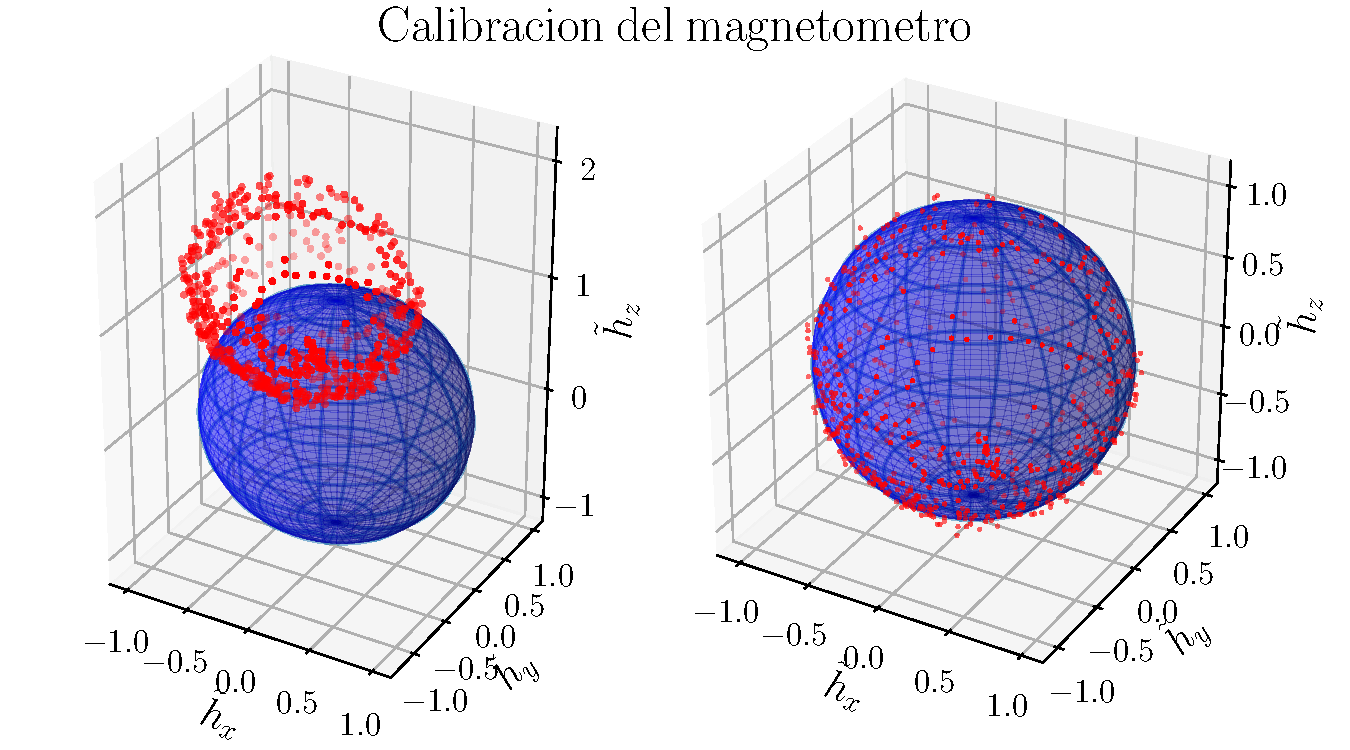
\includegraphics[width=0.9\linewidth]{magnetometer_cal.pdf}
 	\caption{Lugar geométrico de los puntos del espacio descrito por el vector del campo magnético medido por el sensor cuando le se somete a rotaciones aleatorias en las tres direcciones del espacio. A la izquierda se representan las lecturas brutas previas a la calibración y una esfera de radio unitario centrada en el origen. A la derecha se representan esas mismas lecturas tras aplicar la calibración descrita. Las lecturas del magnetómetro se han normalizado con el módulo del vector del campo magnético en Toulouse (ver tabla \ref{tab:vector_magnetico}.) }
 	\label{fig:mag_cal}
\end{figure}

A partir del modelo de error descrito podemos manipular la ecuación \eqref{eq:model_parameters} para aislar el campo magnético $h$ real en ejes cuerpo.
\begin{equation}
    h=A^{-1}(h_m-b) \label{eq:h-subject}
\end{equation}
done $h$ es el vector del campo magnético real en ejes cuerpo y $h_m$ es el vector del campo magnético medido por el sensor y sometido a las diferentes fuentes de error descritas. La calibración consiste en estimar los términos de la matriz $A$ y del vector $b$ para poder corregir las lecturas del sensor empleando la ecuación \eqref{eq:h-subject}. De ahora en adelante, las lecturas del sensor se asumen normalizadas por el módulo del campo magnético de manera que el vector del campo magnético $h$ satisface, 
\begin{equation}
    h^T h = 1 \label{eq:magnitude}
\end{equation}
Substituyendo la ecuación \eqref{eq:h-subject} en \eqref{eq:magnitude}, se obtiene.
\begin{equation}
    (h_m-b)^T (A^{-1})^{T} A^{-1} (h_m-b) = 1 \label{eq:substitute}
\end{equation}
Se por $Q$ el producto $Q = (A^{-1})^T A^{-1}$. Es fácil comprobar que $Q$ es una matriz simétrica ya que es el producto de una matriz multiplicada por su transpuesta. Sustituyendo se obtiene,
\begin{equation}
    (h_m-b)^T Q (h_m-b) = 1 \label{eq:symmetric}
\end{equation}
Expandiendo la ecuación anterior y simplificando se llega a,
\begin{equation}
    h_m^T Q h_m - h_m^T Q b - b^T Q h_m + b^T Q b - 1 = 0 \label{eq:expanded-symmetric}
\end{equation}
dado que $Q$ es una matriz simétrica, $b^T Q h = h^T Q b$. Por tanto, podemos reescribir la ecuación \eqref{eq:expanded-symmetric} como
\begin{equation}
    h_m^T Q h_m - 2h_m^T Q b + b^T Q b - 1 = 0 \label{eq:simplified}
\end{equation}
La ecuación \eqref{eq:simplified} puede finalmente escribirse como la ecuación de una forma cuadŕática
\begin{equation}
    h_m^T Q h_m + h_m^T n + d = 0 \label{eq:quadric}
\end{equation}
donde
\begin{eqnarray}
    Q &= (A^{-1})^T A^{-1} \label{eq:Q-definition}\\
    n &= -2Qb \label{eq:n-definition}\\
    d &= b^T Qb - 1 \label{eq:d-definition}
\end{eqnarray}

El método de calibración del magnetómetro consiste en una calibración tridimensional que emplea el ajuste por mínimos cuadrados y se presenta con detalle en \cite{kok2012calibration, renaudin2010complete, magnusson2013state}. En ausencia de perturbaciones ni errores de desalineamineto, el módulo del vector del campo magnético medido por el sensor debe ser igual al módulo campo magnético terrestre independientemente de la orientación del sensor. En consecuencia, cuando el sensor se gira en los tres ejes del espacio, el vector del campo magnético medido por el sensor en ejes cuerpo debe describir una esfera de radio igual al módulo del vector del campo magnético. Debido a las diferentes fuentes de error descritas anteriormente, la traza del vector del campo magnético obtenida al girar el sensor formará un elipsoide. 


La calibración consiste en encontrar los parámetros $Q$, $n$ y $d$ que satisfacen la ecuación \eqref{eq:quadric}. Se trata de un problema de ajuste de elipsoides utilizando las lecturas del sensor recopiladas para diferentes orientaciones. De entre los diferentes métodos de ajuste de elipsoides existentes es posible citar los algoritmos algebraicos \cite{li2004least, fitzgibbon1999direct}, geométricos \cite{cheng1999statistical} y adaptativos \cite{markovsky2004consistent}. En la presente implementación se ha utilizado la metodología descrita en \cite{li2004least}. 

 La calibración requiere medir el campo magnético en un gran número de orientaciones espaciales diferentes. A diferencia del acelerómetro, que requiere una calibración estática, el magnetómetro puede ser calibrado de forma dinámica, registrando los valores de las lecturas del magnetómetro durante un periodo de tiempo y girando el sensor en las tres direcciones del espacio. No obstante, debido a los ya mencionados errores de hierro duros y suaves, para ser efectiva la calibración debe realizarse directamente en la planta final. Esta operación puede resultar complicada en sistemas reales. Otros métodos de calibración 2D como el presentado por \cite{caruso1998applications} permiten simplificar la fase de adquisición de datos para la calibración.

Tras ajustar los valores de $Q$, $n$ y $d$ utilizando los datos experimentales es posible calcular la matriz $A$ aplicando,
\begin{equation}
    b=-Q^{-1}n
\end{equation}
\begin{equation}
    A^{-1}= \frac{M^{1/2}}{\sqrt{n^{T}M^{-1}n-d}}
\end{equation}






\chapter{Extended Kalman Filter}\label{chapter:EKF}



In order to use the Kalman Filter, we first have to define the states that we want to use. This is why there are so many different kalman filter implementations out there. Every author out there is saying that using their chosen states, you will be able to achieve a better result. However, for the purpose of this tutorial, we are just going to implement a really simple (in comparison to other implementations) one which is similar to the one implemented in my other post for determining a 1 dimensional angle using kalman filter.

Although I said that this is simple relatively, it is actually not that simple. Moving from 2D to 3D is really a big jump as you have to start using vectors and matrices, but that’s not something to be afraid of so let us press on.

The states that we will be using for this implementation is given as follows:
\begin{equation}
    x = \begin{bmatrix} q_0\quad q_1 \quad q_2 \quad q_3 \quad b^g_1 \quad b^g_2 \quad b^g_3 \end{bmatrix}^T
\end{equation}
where

$q_0$ is the scalar term in the quarternion
$q_1$, $q_2$, $q_3$ is the vector term in the quarternion
$b^g_1$,$b^g_2$,$b^g_3$ is the bias of the gyrometer in the $x$, $y$, $z$ direction respectively (units is the same as angular velocity).

The bias term refers to how much the gyrometer would have drifted per unit time. For more information, you can read up my other post for a 1 dimensional kalman filter implementation.

For this implementation, we can write the states in a more concise and compact manner as shown below.
\begin{equation}
    x = \begin{bmatrix} \tilde{q} \\ \tilde{b}^g \end{bmatrix}
\end{equation}
where $\tilde{q}$ is the quaternion and $\tilde{b}^g$ is the bias vector

Now, we need to form an equation for the system dynamics. From section 3, we know that
\begin{equation}
    \dot{q}=\dfrac{1}{2}S(w)q=\dfrac{1}{2}S(q)w
\end{equation}
where
\begin{eqnarray}
    S(w) &=&\begin{bmatrix} 0 & -w_1 & -w_2 & -w_3 \\
                            w_1 &  0 & w_3&  -w_2 \\
                            w_2 & -w_3 & 0 & w_1 \\
                            w_3 & w_2 & -w_1 & 0 \end{bmatrix} \\
    q&=&\begin{bmatrix} q_0 \\ q_1 \\ q_2 \\ q_3\end{bmatrix} \\ 
    S(q)&=&\begin{bmatrix} -q_1 & -q_2 & -q_3 \\ q_0 & -q_3 & q_2 \\ q_3 & q_0 & -q_1 \\ -q_2 & q_1 & q_0 \end{bmatrix} \\
    w &=&\begin{bmatrix} w_1 \\ w_2 \\ w_3\end{bmatrix}
\end{eqnarray}
In order to compensate for the gyrometer bias, we will need to add in the bias term into equation (2).
\begin{eqnarray}
    \dot{q} &=&\dfrac{1}{2}S(w - b^g)q \\ 
    &=& \dfrac{1}{2}S(w)q - \dfrac{1}{2}S(b^g)q \\
    &=& \dfrac{1}{2}\begin{bmatrix} 0 & -w_1 & -w_2 & -w_3 \\ w_1 & 0 & w_3 & -w_2 \\ w_2 & -w_3 & 0 & w_1 \\ w_3 & w_2 & -w_1 & 0 \end{bmatrix}\begin{bmatrix} q_0 \\ q_1 \\ q_2 \\ q_3\end{bmatrix} + \dfrac{1}{2}\begin{bmatrix} 0 & -{b^g}_1 & -{b^g}_2 & -{b^g}_3 \\ {b^g}_1 & 0 & {b^g}_3 & -{b^g}_2 \\ {b^g}_2 & -{b^g}_3 & 0 & {b^g}_1 \\ {b^g}_3 & {b^g}_2 & -{b^g}_1 & 0 \end{bmatrix}\begin{bmatrix} q_0 \\ q_1 \\ q_2 \\ q_3 \end{bmatrix}
\end{eqnarray}

Next, we will need to discretize the above equation so that we can implement it in our program that runs in discrete time. Here, we are simply going to use the first order linearized model to make things simpler. Therefore,
\begin{equation}
    \dot{q}(k) = [q(k+1) - q(k)] / T
\end{equation}
where $T$ is the time taken between sample $k+1$ and $k$. Rearranging the equation,
\begin{equation}
    q(k+1) = T\dot{q}(k) + q(k)
\end{equation}
Substituting equation (3) into equation (4),
\begin{equation}
    q(k+1) = \dfrac{T}{2}S(w)q(k) - \dfrac{T}{2}S(b^g)q(k) + q(k)
\end{equation}
We can actually write equation (4) in a different manner as shown below such that it will be more meaningful when written in matrix form later.
\begin{equation}
    q(k+1) = \dfrac{T}{2}S(q(k))w - \dfrac{T}{2}S(q(k))b^g + q(k)
\end{equation}
Thus, the system state equation can be written as follows.
\begin{eqnarray}
    x_{k+1} &=& \begin{bmatrix} I_{4\times4} & - \dfrac{T}{2}S(q) \\ 0_{3\times4} & I_{3\times3} \end{bmatrix}_kx_k + \begin{bmatrix} \dfrac{T}{2}S(q) \\ 0_{3\times3} \end{bmatrix}_kw_k \\
    \begin{bmatrix} q \\ b^g \end{bmatrix}_{k+1} &=& \begin{bmatrix} I_{4\times4} & - \dfrac{T}{2}S(q) \\ 0_{3\times4} & I_{3\times3} \end{bmatrix}_k\begin{bmatrix} q \\ b^g \end{bmatrix}_k + \begin{bmatrix} \dfrac{T}{2}S(q) \\ 0_{3\times3} \end{bmatrix}_kw_k
\end{eqnarray}
If you expand equation (7), you will find that the first row will resolve into equation (6), and the second row simply says that the bias at time k+1 is the same as the bias at time k. This may look silly at first because we are just saying that the bias is constant. However, the Kalman Filter alters the states of the equation thus the value of the bias actually changes over time when we actually implement the algorithm. For the sake of clarity, I am going to expand equation (7) so that there will be no confusion. Below is the expanded form of equation (7).
\begin{equation}
    \begin{bmatrix} q_0 \\ q_1 \\ q_2 \\ q_3 \\ {b^g}_x \\ {b^g}_y \\ {b^g}_z \end{bmatrix}_{k+1} = \begin{bmatrix} 1 & 0 & 0 & 0 & -\dfrac{T}{2}(-q_1) & -\dfrac{T}{2}(-q_2) & -\dfrac{T}{2}(-q_3) \\ 0 & 1 & 0 & 0 & -\dfrac{T}{2}(q_0) & -\dfrac{T}{2}(-q_3) & -\dfrac{T}{2}(q_2) \\ 0 & 0 & 1 & 0 & -\dfrac{T}{2}(q_3) & -\dfrac{T}{2}(q_0) & -\dfrac{T}{2}(-q_1) \\ 0 & 0 & 0 & 1 & -\dfrac{T}{2}(-q_2) & -\dfrac{T}{2}(q_1) & -\dfrac{T}{2}(q_0) \\ 0 & 0 & 0 & 0 & 1 & 0 & 0 \\ 0 & 0 & 0 & 0 & 0 & 1 & 0 \\ 0 & 0 & 0 & 0 & 0 & 0 & 1 \end{bmatrix} \begin{bmatrix} q_0 \\ q_1 \\ q_2 \\ q_3 \\ {b^g}_x \\ {b^g}_y \\ {b^g}_z \end{bmatrix}_k + \dfrac{T}{2}\begin{bmatrix} -q_1 & -q_2 & -q_3 \\ q_0 & -q_3 & q_2 \\ q_3 & q_0 & -q_1 \\ -q_2 & q_1 & q_0 \\ 0 & 0 & 0 \\ 0 & 0 & 0 \\ 0 & 0 & 0 \end{bmatrix}_k \begin{bmatrix} w_1 \\ w_2 \\ w_3\end{bmatrix}_k
\end{equation}
Before we move on to the actual implementation, let us first take a look at how we can use the accelerometer and magnetometer data in order get the reference vectors. 

\section{Accelerometer data}
The acceleration measured by the accelerometer module can be calculated if we know the acceleration of the body in the world frame, and the orientation of the body. Our reference vector is going to be the gravity vector, and we know that this vector will always point downwards in the world frame. Therefore, if we know the orientation of the body, we can predict the acceleration that the accelerometer is going to measure. This is all based on the assumption that external forces are negligible thus the only force that acts on the body is the gravitational force. As a result of this assumption, you will find that once you move the body hectically, the algorithm will not perform well. There are of course ways to alleviate this problem, but we will not go into there for the purpose of this tutorial.

The above paragraph can be summarized into the following equation.
\begin{equation}
    ^ba_m = ^bR_w(-g) + ^be_a + ^bb_a
\end{equation}
where

$^ba_m$ is the measured acceleration in the body frame by the accelerometer, $^bR_w$ is the rotation matrix for world frame to body frame, $g$ is the gravitational vector in the world frame, $g=\begin{bmatrix} 0 &0 &1\end{bmatrix}_T$, $^be_a$ is the accelerometer noise in the body frame and $^bb_a$ is the accelerometer bias in the body frame

Since we can determine all the variables on the right hand side (except for the noise term), it is possible to predict the measured acceleration. We can then use this prediction to compare with the actual measured acceleration to determine the error in our orientation. The Extended Kalman Filter (EKF) will then automatically help us convert this error into the bias term of the gyrometer. This is what I call the magic of the EKF because I do not need to know how the conversion is done. EKF handles it all as you will see in the later section.

For now, let us define some of the variables above. From the quaternion, it is possible to derive the rotation matrix with the following equation. Do read up on my previous post if you need more information on this.
\begin{equation}
    ^bR_w = {^bR_w}^T = R(q)^T = \begin{bmatrix} q_0^2+q_1^2-q_2^2-q_3^2 & 2(q_1q_2-q_0q_3) & 2(q_1q_3+q_0q_2) \\ 2(q_1q_2+q_0q_3) & q_0^2-q_1^2+q_2^2-q_3^2 & 2(q_2q_3-q_0q_1) \\ 2(q_1q_3-q_0q_2) & 2(q_2q_3+q_0q_1) & q_0^2-q_1^2-q_2^2+q_3^2 \end{bmatrix}^T
\end{equation}

\begin{equation}
    ^bR_w = \begin{bmatrix} q_0^2+q_1^2-q_2^2-q_3^2 & 2(q_1q_2+q_0q_3) & 2(q_1q_3-q_0q_2) \\ 2(q_1q_2-q_0q_3) & q_0^2-q_1^2+q_2^2-q_3^2 & 2(q_2q_3+q_0q_1) \\ 2(q_1q_3+q_0q_2) & 2(q_2q_3-q_0q_1) & q_0^2-q_1^2-q_2^2+q_3^2 \end{bmatrix}
\end{equation}
Since we know that $g=\begin{bmatrix} 0 &0 &1\end{bmatrix}_T$, we can substitute equation (9) into equation (8) and then simplify equation (8) to get the following equation.
\begin{equation}
    \begin{bmatrix} ^ba_x \\ ^ba_y \\ ^ba_z \end{bmatrix} = -\begin{bmatrix} 2(q_1q_3 - q_0q_2) \\ 2(q_2q_3 + q_0q_1) \\ q_0^2 - q_1^2 - q_2^2 + q_3^2 \end{bmatrix} + \begin{bmatrix} ^bb_x \\ ^bb_y \\ ^bb_z \end{bmatrix} + \begin{bmatrix} ^be_x \\ ^be_y \\ ^be_z \end{bmatrix}
\end{equation}
*take note that in the above equation (10), g is a scalar. Notice in equation (10) that the matrix with quaternion terms is non-linear. In order to use the Kalman Filter, we have to write equation (10) in the form of $y=Cx+D$ where $x$ is the state matrix as shown in equation (1) and y is the term on the left hand side of equation (10). You will realize that this is not possible because of the non-linearity. One possible solution is that we can linearize equation (10) near its “operating point”. This is exactly what the Extended Kalman Filter is doing, and also why you need to use the extended form of the Kalman Filter when working with rotation matrices because they are mostly non-linear. So, how do we go about linearizing equation (10)? We can rewrite equation (8), the unexpanded form of equation (10), evaluated at time $t$ as shown below.
\begin{equation}
    (^ba_m)_k = -gh_a(q_k) + C_k
\end{equation}
where $(^ba_m)_k$ is the measured acceleration in the body frame by the accelerometer at time step $k$
$g$ is the gravitational constant (take note that $g$ is a scalar here), $h_a(q_k)$ represents a non-linear function in $q_k$, where $q_k$ is the quaternion at time step $k$, $C_k$ represents the other terms in equation (8), $^be_a+^bb_a$, evaluated at time step $k$.

Just for clarity, I am going to write the values of $h_a(q_k)$ below so that there will be no misunderstandings.
\begin{equation}
    h_a(q_k) = \begin{bmatrix} 2(q_1q_3 - q_0q_2) \\ 2(q_2q_3 + q_0q_1) \\ q_0^2 - q_1^2 - q_2^2 + q_3^2 \end{bmatrix}_k
\end{equation}
With this, what we need to do now becomes much clearer. We have to linearize the nonlinear function $h_a(q_k)$, and one way of doing so is to find its Jacobian (gradient) at time $k-1$. In doing so, we are assuming that the non-linear function is approximately linear between 2 points adjacent in time. This also means that the approximation will be better if you have a shorter timestep between your iterations.

In order to linearize a function, we will call upon the mighty Taylor Expansion as shown below.
\begin{equation}
    f(x)|_{x=a} = f(a) + f^\prime(a)(x-a) + \dfrac{f^{\prime\prime} a)}{2}(x-a)^2 + \ldots
\end{equation}
where $f(x)$ is a non-linear function in $x$. Applying the above to our non-linear function, we will get the following equation.
\begin{equation}
    h_a(q_k)|_{q_k=q_{k-1}} = h_a(q_{k-1}) + h^\prime_a(q_{k-1})(q_k - q_{k-1}) + \ldots
\end{equation}
where,
\begin{equation}
    h^\prime_a(q_{k-1}) = \dfrac{\delta{h_a(q)}}{\delta{q}}|_{q=q_{k-1}} = \begin{bmatrix} \dfrac{\delta{h_{a1}}}{\delta{q_0}} & \dfrac{\delta{h_{a1}}}{\delta{q_1}} & \dfrac{\delta{h_{a1}}}{\delta{q_2}} & \dfrac{\delta{h_{a1}}}{\delta{q_3}} \\ \dfrac{\delta{h_{a2}}}{\delta{q_0}} & \dfrac{\delta{h_{a2}}}{\delta{q_1}} & \dfrac{\delta{h_{a2}}}{\delta{q_2}} & \dfrac{\delta{h_{a2}}}{\delta{q_3}} \\ \dfrac{\delta{h_{a3}}}{\delta{q_0}} & \dfrac{\delta{h_{a3}}}{\delta{q_1}} & \dfrac{\delta{h_{a3}}}{\delta{q_2}} & \dfrac{\delta{h_{a3}}}{\delta{q_3}} \end{bmatrix}_{k-1}
\end{equation}
\begin{equation}
    h^\prime_a(q_{k-1}) = 2\begin{bmatrix} -q_2 & q_3 & -q_0 & q_1 \\ q_1 & q_0 & q_3 & q_2 \\ q_0 & -q_1 & -q_2 & q_3 \end{bmatrix}_{k-1}
\end{equation}
And there we have it! Let us now substitute equation (13) into equation (12).
\begin{equation}
    h_a(q_k)|_{q_k=q_{k-1}} = \begin{bmatrix} 2(q_1q_3 - q_0q_2) \\ 2(q_2q_3 + q_0q_1) \\ q_0^2 - q_1^2 - q_2^2 + q_3^2 \end{bmatrix}_{k-1} + 2\begin{bmatrix} -q_2 & q_3 & -q_0 & q_1 \\ q_1 & q_0 & q_3 & q_2 \\ q_0 & -q_1 & -q_2 & q_3 \end{bmatrix}_{k-1} \left( \begin{bmatrix} q_0 \\ q_1 \\ q_2 \\ q_3 \end{bmatrix}_k - \begin{bmatrix} q_0 \\ q_1 \\ q_2 \\ q_3 \end{bmatrix}_{k-1} \right)
\end{equation}
Now that we have the linearized form of the non-linear equation, let us write out the whole linearized solution of equation (10).
\begin{equation}
    \begin{bmatrix} ^ba_x \\ ^ba_y \\ ^ba_z \end{bmatrix}_k = -g\left[ \begin{bmatrix} 2(q_1q_3 - q_0q_2) \\ 2(q_2q_3 + q_0q_1) \\ q_0^2 - q_1^2 - q_2^2 + q_3^2 \end{bmatrix}_{k-1} + 2\begin{bmatrix} -q_2 & q_3 & -q_0 & q_1 \\ q_1 & q_0 & q_3 & q_2 \\ q_0 & -q_1 & -q_2 & q_3 \end{bmatrix}_{k-1} \left( \begin{bmatrix} q_0 \\ q_1 \\ q_2 \\ q_3 \end{bmatrix}_k - \begin{bmatrix} q_0 \\ q_1 \\ q_2 \\ q_3 \end{bmatrix}_{k-1} \right) \right] + \begin{bmatrix} C_x \\ C_y \\ C_z \end{bmatrix}_k
\end{equation}
Take note that $g$ is a scalar term here. In the Python source code, you will notice that the $C_k$ matrix is missing. This is because I calibrated the accelerometer at first to deal with the bias. In other words, I was working with a $0$ bias accelerometer value so the $C_k$ term becomes $0$.

Let us now write equation (15) in a more compact matrix form so that it will be clearer.
\begin{equation}
    y=Cx+D
\end{equation}
where
\begin{equation}
    y = (^ba_m)_k =\begin{bmatrix} ^ba_x \\ ^ba_y \\ ^ba_z \end{bmatrix}_k
\end{equation}
\begin{equation}
    C= -g[2h^\prime_a(q_{k-1})] =-2g\begin{bmatrix} -q_2 & q_3 & -q_0 & q_1 \\ q_1 & q_0 & q_3 & q_2 \\ q_0 & -q_1 & -q_2 & q_3 \end{bmatrix}_{k-1}
\end{equation}
\begin{equation}
    x = q_k =\begin{bmatrix} q_0 \\ q_1 \\ q_2 \\ q_3 \end{bmatrix}_k
\end{equation}
(here, the bias terms in equation (1) are treated as zeros)
\begin{eqnarray}
    D &=& -g[h_a(q_{k-1}) - 2h^\prime_a(q_{k-1})(q_{k-1}) + C_k] \\
    &=& -g\left[\begin{bmatrix} 2(q_1q_3 - q_0q_2) \\ 2(q_2q_3 + q_0q_1) \\ q_0^2 - q_1^2 - q_2^2 + q_3^2 \end{bmatrix}_{k-1} - 2\begin{bmatrix} -q_2 & q_3 & -q_0 & q_1 \\ q_1 & q_0 & q_3 & q_2 \\ q_0 & -q_1 & -q_2 & q_3 \end{bmatrix}_{k-1}\begin{bmatrix} q_0 \\ q_1 \\ q_2 \\ q_3 \end{bmatrix}_{k-1} +\begin{bmatrix} C_x \\ C_y \\ C_z \end{bmatrix}_k \right]
\end{eqnarray}
We now have a system of linear equations, albeit being a little ugly. Actually, in the kalman filter implementation, we are only going to use matrix $C$ (the Jacobian matrix) thus the rest of the terms are actually not needed. There are some mathematical proofs for this, but that is beyond the scope of this tutorial. We are now finally done with the accelerometer section.
\section{Magnetometer data}

The magnetometer provides us with a vector that is always pointing to the magnetic North. This vector changes (elevation of the vector changes depending on the altitude) over the surface of the Earth thus we will need a map of the vectors if we want a reference vector that works across the globe. However, in this project, we will be assuming that the change in the North reference vector is negligible since the sensor will not be moving around much (probably only within the room).

The magnetometer actually gives a 3 directional reference vector instead of a simple North heading in 2 dimensions. Due to this, there are some complications that arise. In this project, I will make the assumption that the accelerometer is accurate in providing the reference vector in the vertical plane, and the magnetometer data is accurate in providing the reference vector in the horizontal place. As a result of this, we do not want the magnetometer data to affect the accelerometer data and vice versa. Therefore, we are going to remove 1 dimension from the magnetometer reference vector.

Firstly, we will calibrate our magnetometer based on my previous post so that we can get a 3 dimensional unit vector from the raw magnetometer data. If you follow the method in the previous post, you should be able to determine the values of $A^{-1}$ and $b$ so you can apply the calibration equation as follows.
\begin{equation}
   h=A^{-1}(h_m - b) 
\end{equation}

where $h$ is the actual magnetic field and $h_m$ is the measurement reading from the magnetometer with errors. Next, in order to remove 1 dimension (the vertical plane) from the magnetometer vector, we have to transform the coordinates from the body frame (measurements are done in the body frame) to the world frame first (because the vertical plane that we want to remove exist in the world frame). Therefore, we have to get the rotation matrix that converts the body frame to the world frame from our quaternion. This can be done through equation (1) from my previous post which is shown below as well.
\begin{equation}
    r^\prime=Cr
\end{equation}
where
\begin{equation}
    C=\begin{bmatrix} q_0^2+q_1^2-q_2^2-q_3^2 & 2(q_1q_2-q_0q_3) & 2(q_1q_3+q_0q_2) \\ 2(q_1q_2+q_0q_3) & q_0^2-q_1^2+q_2^2-q_3^2 & 2(q_2q_3-q_0q_1) \\ 2(q_1q_3-q_0q_2) & 2(q_2q_3+q_0q_1) & q_0^2-q_1^2-q_2^2+q_3^2 \end{bmatrix}
\end{equation}
In this case, $r$ will be the unit vector calibrated magnetometer data in the body frame. Therefore,
\begin{equation}
   r = \begin{bmatrix} ^bm_1 \\ ^bm_2 \\ ^bm_3 \end{bmatrix} \qquad r^\prime = \begin{bmatrix} ^wm_1 \\ ^wm_2 \\ ^wm_3 \end{bmatrix}
\end{equation}
$^bm_1$, $^bm_2$, $^bm_3$  is the calibrated magnetometer data in the body frame’s $x$, $y$, $z$ direction respectively.\\

$^wm_1$, $^wm_2$, $^wm_3$ is the calibrated magnetometer data in the world frame’s $x$, $y$, $z$ direction respectively.

Now, we can safely remove the $z$-axis from our data by letting $^wm_3=0$, then re-normalizing the vector such that it stays as a unit vector but only in 2 dimensions now. We will then rotate it back to the body frame and use the resulting vector (in place of the actual calibrated measured data) for our kalman filter update section later on. On a side note, you will find that even without doing all these, the kalman filter algorithm will work. However, whether it works better with or without is another story to be told another day.

In the accelerometer section, we have the gravity vector as our reference vector. On the other hand, we have the North vector as a reference for our magnetometer. For me, since the North vector points exactly in the direction of the negative y-axis when I placed the sensor parallel to my table, I simply took the negative y-axis (in the world frame) as my reference vector. A better approach would be perhaps to have a period of time for the initialization process to set the current North vector as the reference vector. In this way, all we have to do is place the object in the desired direction for it to use the direction as a reference for calculation.

As a result of setting the y-axis to be the reference vector, in place of $g=\begin{bmatrix} 0 &0 &1\end{bmatrix}_T$,, I have $m=\begin{bmatrix} 0 &-1 &0\end{bmatrix}_T$. (in the python code, i added in the negative sign into the gravity reference vector).

Moving on, once again, we need a linear equation for the output of our system in order for us to use the kalman filter. The output that we want to get here is the predicted accelerometer and magnetometer data from our kalman filter states (quaternion). One way of doing so is through the rotation matrix which can be derived from a quaternion. Similar to the accelerometer, we can use the following equation to convert the magnetometer reading from the world frame to the body frame (so that we can compare it to the actual measured magnetometer value).
\begin{equation}
    ^bm_m = ^bR_w(^wm_r) + ^be_{mag} + ^bb_{mag}
\end{equation}
where

$^bm_m$ is the measured magnetic field in the body frame by the magnetometer
$^bR_w$ is the rotation matrix for world frame to body frame
$^wm_r$ is the reference magnetic North vector in the world frame, where in my case $^wm_r=\begin{bmatrix} 0 &-1 &0\end{bmatrix}_T$
$^be_{mag}$ is the magnetometer noise in the body frame
$^bb_{mag}$ is the magnetometer bias in the body frame

The rotation matrix $^bR_w$ is actually the same matrix as what was used in the accelerometer. Below is the exact same equation (9).
\begin{equation}
    ^bR_w = \begin{bmatrix} q_0^2+q_1^2-q_2^2-q_3^2 & 2(q_1q_2+q_0q_3) & 2(q_1q_3-q_0q_2) \\ 2(q_1q_2-q_0q_3) & q_0^2-q_1^2+q_2^2-q_3^2 & 2(q_2q_3+q_0q_1) \\ 2(q_1q_3+q_0q_2) & 2(q_2q_3-q_0q_1) & q_0^2-q_1^2-q_2^2+q_3^2 \end{bmatrix}
\end{equation}
Since we know that $^wm_r=\begin{bmatrix} 0 &-1 &0\end{bmatrix}_T$, we can substitute equation (9) into equation (16) and then simplify equation (16) to get the following equation.

\begin{equation}
    \begin{bmatrix} ^bm_x \\ ^bm_y \\ ^bm_z \end{bmatrix} = -\begin{bmatrix} 2(q_1q_2+q_0q_3) \\ q_0^2-q_1^2+q_2^2-q_3^2 \\ 2(q_2q_3-q_0q_1) \end{bmatrix} + \begin{bmatrix} ^bb_x \\ ^bb_y \\ ^bb_z \end{bmatrix} + \begin{bmatrix} ^be_x \\ ^be_y \\ ^be_z \end{bmatrix} 
\end{equation}

From here, you can see that in order to obtain the Jacobian matrix for use in the Extended Kalman Filter, the steps are exactly the same as that for the accelerometer. As such, I am going to skip the derivations and just write down the value of the $C$ matrix below here.

\begin{equation}
    C= -2\begin{bmatrix} q_3 & q_2 & q_1 & q_0 \\ q_0 & -q_1 & q_2 & -q_3 \\ -q_1 & -q_0 & q_3 & q_2 \end{bmatrix}_{k-1}
\end{equation}
Here, notice that if we did not simplify the equations with the values of wmr for equation (16), we will get the exact same generalized Jacobian matrix from equation (8) (without the values of the vector g being substituted) as well. I will leave this as homework to you guys but the answer can be found in the python code anyway. I was lazy to write 2 different implementations for the accelerometer and the magnetometer so I combined them both. Anyway, we are now ready to get on with the EKF implementation finally!
\section{Quaternion EKF Implementation}

The equations that we are going to implement are exactly the same as that for the kalman filter as shown below. (This is taken directly from my earlier post except that i added k to the numbering to symbolize that it is the kalman filter equation)

Prediction

\begin{equation}
    \hat{x}^-_k=A\hat{x}_{k-1}+Bu_k
\end{equation}
\begin{equation}
    P^-_k=AP_{k-1}A^T+Q
\end{equation}


where $\hat{x}_k^{-}$ is the priori estimate of $x$ at time step $k$, $P^-_k$ is the priori estimate of the error at time step $k$ and $Q$ is the process variance.

Update
\begin{equation}
    K_k=\frac{P^-_kC^T}{CP^-_kC^T+R}
\end{equation}
\begin{equation}
    \hat{x}_k=\hat{x}^-_k+K_k(y_k-C\hat{x}^-_k)
\end{equation}
\begin{equation}
    P_k=(I-K_kC)P^-_k
\end{equation}
where $y_k$ is the actual measured state, $\hat{x}_k$ is the posteri estimate of $x$ at time step $k$, $P_k$ is the posteri estimate of the error at time step $k$, $K_k$ is the kalman gain at time step $k$ and $R$ is the measurement variance. Let us go through the equations in order.


\subsection{Prediction}

\subsubsection{Equation 1K}
\begin{equation}
    \hat{x}_{k}^- = A\hat{x}_{k-1} + Bu_k
\end{equation}
If you know the kalman filter well, you would have realized that we have derived this equation already in the earlier part of this post. Below is a copy of the equation (7) from the kalman filter states section above except that I replace $k$ with $k-1$.
\begin{equation}
    \begin{bmatrix} q \\ b^g \end{bmatrix}_{k} = \begin{bmatrix} I_{4\times4} & - \frac{T}{2}S(q) \\ 0_{3\times4} & I_{3\times3} \end{bmatrix}_{k-1}\begin{bmatrix} q \\ b^g \end{bmatrix}_{k-1} + \begin{bmatrix} \frac{T}{2}S(q) \\ 0_{3\times3} \end{bmatrix}_{k-1}w_{k-1}
\end{equation}
From the above equation, we can determine our $A$ and $B$ matrices.
\begin{equation}
    A=\begin{bmatrix} I_{4\times4} & - \frac{T}{2}S(q) \\ 0_{3\times4} & I_{3\times3} \end{bmatrix}_{k-1}
\end{equation}
\begin{equation}
    B=\begin{bmatrix} \frac{T}{2}S(q) \\ 0_{3\times3} \end{bmatrix}_{k-1}
\end{equation}
where
\begin{equation}
    S(q)=\begin{bmatrix} -q_1 & -q_2 & -q_3 \\ q_0 & -q_3 & q_2 \\ q_3 & q_0 & -q_1 \\ -q_2 & q_1 & q_0 \end{bmatrix}
\end{equation}
With all these information, we can now determine $\hat{x}^{-}_{k}$ in equation (1K). Once this is done, we have to normalize the quaternion in our kalman filter states dues inaccuracies in the discretized calculation. Next up is equation (2k).

\subsubsection{Equation 2K}

\begin{equation}
    P^-_k=AP_{k-1}A^T+Q
\end{equation}
This equation is pretty straightforward. However, we have to decide an initial value for the $P$ matrix and the $Q$ matrix. You should play around with the values in the code to see how this affects the overall performance of the algorithm. You will realize that if you start with a $P$ matrix with huge values, it may not converge to give you a coherent result. On the other hand, if you start with a $P$ matrix with small values, it may take quite a while for the $P$ matrix to converge to the actual solution. The Q matrix is the process variance, and it represents the inaccuracies of the model that we are using.

In the code, equation (1k) and (2k) are both done within the predict() method as shown below. (predictAccelMag() will be explained under equation (3k))

\subsection{Update}

\subsubsection{Equation 3K}

\begin{equation}
    K_k=\frac{P^-_kC^T}{CP^-_kC^T+R}
\end{equation}

In order to implement equation (3k), we first have to figure out what is our $C$ matrix here. If you take a look at my previous post explaining the kalman filter using the pendulum example, you will know that the $C$ matrix is a matrix to convert our kalman filter states to the measured variables. In the pendulum example, it just so happens that the measured variables are the same as the kalman filters states thus the $C$ matrix is the identity matrix. However, in our case here, our measured variables are the direction of the gravity and North vector while our kalman filter states are the quartenion and the gyro bias. They are essentially different parameters thus we have to figure out a $C$ matrix which allows us to convert out state variables into the measured variables.

Now, if you had diligently read through everything in this post, you should realize that we have already derived our $C$ matrix in the accelerometer and magnetometer section. For the Accelerometer,
\begin{equation}
    C_a= -2\begin{bmatrix} -q_2 & q_3 & -q_0 & q_1 \\ q_1 & q_0 & q_3 & q_2 \\ q_0 & -q_1 & -q_2 & q_3 \end{bmatrix}_{k-1}
\end{equation}
Notice here that I removed the multiple $g$ because the accelerometer data that I will be using is in units of $g$. For the Magnetometer,
\begin{equation}
    C_m= -2\begin{bmatrix} q_3 & q_2 & q_1 & q_0 \\ q_0 & -q_1 & q_2 & -q_3 \\ -q_1 & -q_0 & q_3 & q_2 \end{bmatrix}_{k-1}
\end{equation}
In order to determine the $C$ matrix, we would require the quaternion state from the previous iteration. Since the conversion of quaternion to rotation matrix from the world frame to the body frame is the same for the accelerometer and the magnetometer, there is actually a more generalized form of the $C$ equation that will work for both the accelerometer and the magnetometer. I left that as a homework in the above section but the answer is actually already within the code under the method getJacobianMatrix(). For the purpose of clarity, I am once again going to write out the exact equation that is implemented within the python code.

\begin{eqnarray}
    \hat{y}^-_k &=& C\hat{x}^-_k \\ 
    \begin{bmatrix} \hat{a}_m \\ \hat{m}_m \end{bmatrix}_k &=& \begin{bmatrix} C_a & 0_{3\times3}  \\ C_m & 0_{3\times3} \end{bmatrix} \begin{bmatrix} q \\ b^g \end{bmatrix}_k 
\end{eqnarray}
The last term that we have to determine in order to implement equation (3k) is the $R$ matrix. This is the measurement variance and it represents how accurate our measurement data is. Similar to the $Q$ matrix in equation (2k), this term is important yet difficult to determine. The values of these terms are usually determine through simulations or actual tests so in this tutorial, I am just going to use an arbitrary value which does not have any special meaning.


\subsubsection{Equation 4K}

\begin{equation}
    \hat{x}_k=\hat{x}^-_k+K_k(y_k-C\hat{x}^-_k)
\end{equation}
Next up is equation (4k) which by now we should have all the terms except for $y_k$. This is the actual measurement values that we obtain from the sensor data. In my python code, this is expressed as shown below.
\begin{equation}
    y_k = \begin{bmatrix} a_m \\ m_m \end{bmatrix}
\end{equation}
Since we are making an addition to the quaternion, we have to normalize it again after this step to maintain a unit quaternion during the calculations.

\subsubsection{Equation 5K}

\begin{equation}
    P_k=(I-K_kC)P^-_k
\end{equation}

As for equation (5k), we already have all the variables ready so implementing it will be no problem at all. Equation (3k) to (5k) are all implemented within the update() method in the python code as shown below as well.



\appendix
\newpage
\nocite{*}

% \bibliography{references}
\printbibliography

\end{document} 